%%%%%%%%%%%%%%%%%%%%%%%%%%%%%%%%%%%%%%%%%
% University Assignment Title Page 
% LaTeX Template
% Version 1.0 (27/12/12)
%
% This template has been downloaded from:
% http://www.LaTeXTemplates.com
%
% Original author:
% WikiBooks (http://en.wikibooks.org/wiki/LaTeX/Title_Creation)
%
% License:
% CC BY-NC-SA 3.0 (http://creativecommons.org/licenses/by-nc-sa/3.0/)
% 
% Modified for COSC480/490 by:
% Lech Szymanski (8/3/18)
%
% Modified for Eden's COSC385 report. (09/2025)

% texcount -inc -sum -sub=section myreport.tex

\documentclass[12pt]{article}
\usepackage[draft]{cosc4x0style}
\usepackage{float}
\usepackage{tikz}
\usepackage{wrapfig}
\usepackage{changepage}
\usepackage{listings}
\usepackage{caption}
\usepackage[edges]{forest}
\usepackage{amsmath}
\usepackage{amssymb}
\usepackage{amsfonts}
\usetikzlibrary{shapes,arrows,positioning,shapes.multipart,arrows.meta,fit,backgrounds,arrows.meta,calc,decorations.pathreplacing}

\tikzset{
  >={Stealth[length=2mm,width=2mm]},
  neuron/.style={circle,draw,minimum size=12mm,inner sep=0pt},
  tanhNeuron/.style={
    neuron,
    path picture={
      \begin{scope}
        % Draw a symmetrical S-like tanh curve with visible flat ends
        \clip (path picture bounding box.south west)
              rectangle (path picture bounding box.north east);
        \draw[line width=0.8pt, samples=40, domain=-1.2:1.2, smooth]
          plot (\x*3mm, {1.8mm*tanh(1.6*\x)});
      \end{scope}
    }
  },
  linearNeuron/.style={
    neuron,
    path picture={
      % straight line to denote linear logits
      \draw[line width=0.8pt]
        (path picture bounding box.south west)++(2mm,2mm)
        -- (path picture bounding box.north east)++(-2mm,-2mm);
    }
  },
  inDot/.style={circle,fill=black,minimum size=3mm,inner sep=0pt},
  layerlabel/.style={font=\small,anchor=south},
}

% To compile the final version of the report (which will remove all the todo content)
%\usepackage{cosc4x0style}

% Specify project code 480 or 490
\papercode{385}

% Your project title
\title{Talking in French Like Academia\\\large Mistral 7B Powered Verlan Identification}

% Your name
\author{Yitian \textsc{Li}}
\studentid{4556502}

% Names of your supervisors, separated by line break '\\'
\supervisors{
  Dr Lech \textsc{Szymanski} \\
  Dr Veronica \textsc{Liesaputra}
}

% Date, change the \today to a set date if you want to be precise
\reportdate{\today}

\begin{document}


\maketitle

\begin{abstract}
something.
\end{abstract}
% Need abstract in French!
%need glossary and acknowledgements

\section{Introduction}
\subsection{Context and Motivation}

Since the early 19th century, the French people have started to talk using verlan. Just like Pig Latin\footnote{\url{en.wikipedia.org/wiki/Pig_Latin}} exists in English culture, verlan is an unusual and creative form of \textit{argot} (slang) that is formed by flipping the syllables around in a word.\footnote{In fact, the word \textit{verlan} is a verlan from the word \textit{l'inver} (the inversion).}\cite{rajabov2025,bach2018} 
Time flies, verlan has become more and more popular, and it is now widely used amongst teens and young people in francophone societies\footnote{Such as France, Belgium, Switzerland, Luxembourg, and Canada.}\cite{evolutionverlan}. Examples of verlan can be as follows:

\begin{flushleft}
\small
\begin{itemize}
  \item bite = bi + te \(\rightarrow\) te + bi \(\rightarrow\) tebie (penis)
  \item shit = shi + t \(\rightarrow\) t + shi \(\rightarrow\) teuchi\cite{evolutionverlan}
  \item bonjour = bon + jour \(\rightarrow\) jour + bon \(\rightarrow\) jourbon (greetings)
\end{itemize}
\end{flushleft}

\noindent In real-life conversations, such can be used as in the example sentences below:

\begin{flushleft}
\small
\begin{itemize}
  \item \textit{Le graff géant représente une tebie pixel art.}\\(The giant graffiti depicts a pixel art penis.)
  \item \textit{Il a du bon teuchi du bled.}\\(He's got some good shit from the countryside.)
  \item \textit{Un p'tit\footnote{Standard spelling: petit.}jourbon et tout le monde sourit.}\\(A quick hello and everyone smiles.)
\end{itemize}
\end{flushleft}

Indeed, verlan can be formed with different original languages, not only French, but also English and other languages. However, it always follows the same rule of flipping syllables, although, for better pronunciation reasons, certain minor amendments such as dropping unnecessary letters and applying accents (e.g., é, è) can be used from time to time\cite{rajabov2025}. Besides, due to the universal trait of slang being used more often phonetically instead of written, verlan users tend to spell them differently when writing them down. As technology develops, this has been occurring more frequently than ever in daily texting\cite{rua2005}.

Thinking internationally, when people are communicating with translators, it is possible that slang in their mother language can be brought to the conversation, which could be tricky for translators to translate\cite{hajiyeva2025}. Using translators such as DeepL\footnote{\url{www.deepl.com}} and Google Translate\footnote{\url{translate.google.com}} to translate sentences that contain verlan from French to English can be a specific example to prove this. Furthermore, although both of the translators above are using Machine Learning (ML) for translation, their results of translating verlans are not ideal\cite{deepl2020, wu2016}. For example, when attempting to translate the sentence above, \textit{Le graff géant représente une tebie pixel art.}, both Google Translate\ref{fig:google_verlan} and DeepL\ref{fig:deepl_verlan} cannot translate the word \textit{tebie} correctly. Specifically, for DeepL, there is no desired translation as \textit{penis} in its alternative word list for \textit{tebie}\ref{fig:deepl_alt_text}.

\begin{figure}[H]
\centering

\includegraphics[width=0.8\textwidth]{figures/google_verlan.png}
\caption{\label{fig:google_verlan}Google Translate cannot translate the verlan \textit{tebie} correctly.}
\end{figure}

\begin{figure}[H]
\centering

\includegraphics[width=0.8\textwidth]{figures/deepl_verlan.png}
\caption{\label{fig:deepl_verlan}DeepL cannot translate the verlan \textit{tebie} correctly.}
\end{figure}

\begin{figure}[H]
\centering

\includegraphics[width=0.3\textwidth]{figures/deepl_alt_text.png}
\caption{\label{fig:deepl_alt_text}No desired translation for verlan \textit{tebie} in DeepL's alternative word list.}
\end{figure}

Thus, a question shall naturally arise: Can we improve translators' performance in translating slang by improving the ML model? The answer is undoubtedly `yes' in an era where artificial intelligence research is expanding rapidly. Researchers have been making progress in identifying slang using ML\cite{pei2019slang} and, moreover, in translating noisy text, of which slang is a part\cite{michel2018mtnt}. 

But what about verlan? There is no known ongoing or completed research on identifying \textit{such} slang or their translations\footnote{Until September 2025.}, nor does a proper dataset exist. The only work similar to this is an assignment published at the University of Toronto\footnote{\url{https://uoft-csc413.github.io/2022/assets/assignments/PA03.pdf}}, asking students to train a Neural Machine Translation (NMT) model to transform standard English into Pig Latin. It is not only the other way around; instead of identifying Pig Latin and transforming it back to standard English, it is also more of an example for students to practice using NMT than a discussion on its identification and translation. Shouldn't we do something?

This report aims to change that.

\subsection{Objective}

The purpose of the project is to create two verlan datasets: one functioning as a dictionary, containing the verlan words and their normalised standard French equivalents; the other a dataset of sentences that contain verlan, paired with the same sentences containing normalised words, with labels indicating whether a sentence contains verlan. After that, the project embeds and classifies verlan using Large Language Models (LLMs) and analyses the results.

\begin{figure}[H]
\centering
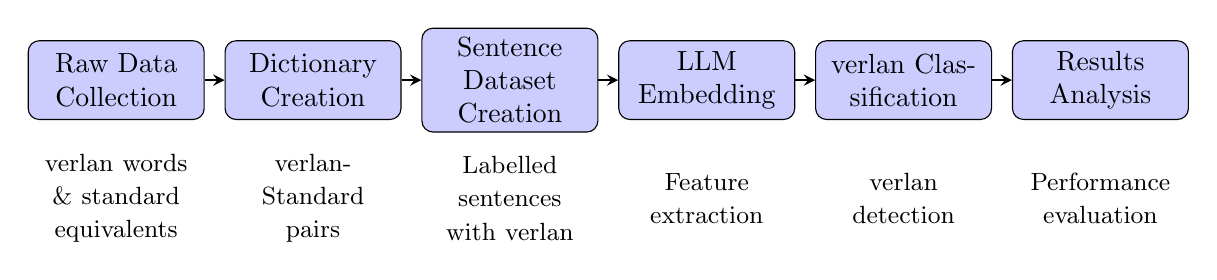
\begin{tikzpicture}[
    node distance=2.5cm,
    auto,
    block/.style={rectangle, draw, fill=blue!20, text width=2cm, text centered, rounded corners, minimum height=1cm},
    arrow/.style={thick,->,>=stealth}
]

% Define nodes from left to right
\node [block] (data) {Raw Data Collection};
\node [block, right of=data] (dict) {Dictionary Creation};
\node [block, right of=dict] (sentences) {Sentence Dataset Creation};
\node [block, right of=sentences] (embedding) {LLM Embedding};
\node [block, right of=embedding] (classification) {verlan Classification};
\node [block, right of=classification] (analysis) {Results Analysis};

% Draw arrows
\draw [arrow] (data) -- (dict);
\draw [arrow] (dict) -- (sentences);
\draw [arrow] (sentences) -- (embedding);
\draw [arrow] (embedding) -- (classification);
\draw [arrow] (classification) -- (analysis);

% Add labels below nodes
\node [below of=data, node distance=1.5cm, text width=2cm, text centered] {\small verlan words \& standard equivalents};
\node [below of=dict, node distance=1.5cm, text width=2cm, text centered] {\small verlan-Standard pairs};
\node [below of=sentences, node distance=1.5cm, text width=2cm, text centered] {\small Labelled sentences with verlan};
\node [below of=embedding, node distance=1.5cm, text width=2cm, text centered] {\small Feature extraction};
\node [below of=classification, node distance=1.5cm, text width=2cm, text centered] {\small verlan detection};
\node [below of=analysis, node distance=1.5cm, text width=2cm, text centered] {\small Performance evaluation};

\end{tikzpicture}
\caption{\label{fig:pipeline}A visulisation of the objectives.}
\end{figure}

With the purpose above, the report contributes to the linguistics and the AI researchers two verlan datasets, for dictionary making or LLMs training. The report also evaluates how good we can achieve the identification of verlan with ML, to benefit machine translation in the future.

The code and the unannotated, un peer-reviewed dataset developed as part of the project are released under openlicences and aligns with open science best practices, with the usage of a version controlled software development platform (GitHub)\footnote{\url{github.com/greateden/verlan-Identification-Normalisation}}. The annotated, peer-reviewed dataset will be published shortly after this report, aiming by the end of 2025.

\section{Background}
\subsection{A Living Verlan}

Vivienne Véla, a former scholar from Université Paris 8, poetically captured one of Verlan's most important traits: it pursues confusion instead of clarity\cite{mela1991verlan}. One reason is that it is widely used among lower-class people, drug users, gangs, or those in jail. Thus, making the context unidentifiable is important\;---\;certain phenomena such as reverlanisation (flipping the Verlan again if it becomes too popular) and truncation are therefore applied. However, although Verlan is used for concealing meaning, it still follows certain rules. The most general rule is syllabic reversal, as mentioned in the introduction chapter of this report.

Specifically, to delve into the linguistic rules, Véla pointed out that the analytic model proposed by Kaye and Lowenstamm provides the best description\cite{kaye1984syllabicite}. The syllable can be disassembled into \textit{attaque} (onset), \textit{rime} (rhyme), \textit{noyau} (nucleus), and \textit{coda}. For example, here is a representation of the word \textit{garder}, IPA\footnote{International Phonetic Alphabet, \url{https://en.wikipedia.org/wiki/International_Phonetic_Alphabet}} [garde].

\begin{figure}[H]
\centering
\begin{forest}
for tree={
  grow=south,
  parent anchor=south,
  child anchor=north,
  align=center,
  edge={-latex},
  l sep=10pt,
  s sep=18pt,
  font=\itshape
}
[{\textbf{garder}}
  [{$S_1$}
    [attaque
      [g, font=\normalfont]
    ]
    [rime
      [noyau
        [a, font=\normalfont]
      ]
      [coda
        [r, font=\normalfont]
      ]
    ]
  ]
  [{$S_2$}
    [attaque
      [d, font=\normalfont]
    ]
    [rime
      [noyau
        [e, font=\normalfont]
      ]
    ]
  ]
]
\end{forest}
\end{figure}

It has two syllables, $S_1$ and $S_2$. To create the Verlan form, we follow the permutation equation below:

\begin{equation}\label{eq:verlan-perm}
  (S_1 S_2) \rightarrow (S_2 S_1)
\end{equation}

After the permutation, we obtain the Verlan form of \textit{garder} as \textit{degar}, represented below.

\begin{figure}[H]
\centering
\begin{forest}
for tree={
  grow=south,
  parent anchor=south,
  child anchor=north,
  align=center,
  edge={-latex},
  l sep=10pt,
  s sep=18pt,
  font=\itshape
}
[{\textbf{degar}}
  [{$S_2$}
    [attaque
      [d, font=\normalfont]
    ]
    [rime
      [noyau
        [e, font=\normalfont]
      ]
    ]
  ]
  [{$S_1$}
    [attaque
      [g, font=\normalfont]
    ]
    [rime
      [noyau
        [a, font=\normalfont]
      ]
      [coda
        [r, font=\normalfont]
      ]
    ]
  ]
]
\end{forest}
\end{figure}

Notably, the permutation occurs only at the syllable level (i.e., between $S_1$ and $S_2$); it does not affect the internal structure of each syllable tree, although in some cases, certain letters (such as \textit{e}) might be dropped after permutation. That said, the example above is not an exhaustive explanation of forming a Verlan. To avoid confusing the readers, this report suggests that this example perfectly illustrates its regular rule. For further details, readers are advised to consult Véla's paper.

With such a sub-word permutation, researchers can not only discuss it within the linguistic realm, but it is also intriguing for computer scientists to explore how machines, such as LLMs, perceive this kind of difference. Just as Véla describes Verlan\;---\;ambiguous, sometimes violent, sometimes amazing, and always vivid.


\subsection{Detecting Slang}

To the best of our knowledge, there is no existing computational research\footnote{As of September 2025.} on the \textit{detection} of Verlan\;---\;this particular form of French slang. However, there are a few scholars who have included Verlan in their research\cite{zurbuchen2024, podhorna2020rapcor, mekki2021tremolo, panckhurst202088milsms}. Yet, these studies commonly included Verlan as a type of slang in their datasets or corpora. Moreover, they did not specifically focus on how to detect this particular type of slang, but rather approached it in a broader sense\;---\;they created slang datasets that contain Verlan, and some of them employed computational approaches to detect such slang.

Fortunately, there are several papers related to computational slang detection, and their approaches could contribute to Verlan detection to a large extent\cite{pei2019slang, sun2024informal, slangornot2024, wu2018slangsd}. These studies are not limited to French but also cover other Indo-European languages\footnote{For example, English, German, and Russian. For more information, please refer to: \url{https://en.wikipedia.org/wiki/Indo-European_languages}.}.

Therefore, regarding the history of Verlan detection, this report first generalises the task as slang detection, and then discusses possible methods that could be implemented for Verlan identification, in order to provide readers with a general and useful background.

\subsubsection{1910s-2016: A Super-Condensed History of Slang Detection}

The background of traditional slang detection often leverages fuzzy-matching methods. Two main methods were introduced and widely cited: Soundex, a phonetic indexing system for names introduced by Russell in 1918, and the edit-distance-based spelling-correction method introduced by Levenshtein in 1966\cite{russell1918soundex, levenshtein1966}. Afterwards, scholars introduced more algorithms, such as Philips's Metaphone and Double Metaphone, which improved on Russell's Soundex; Kukich's methods for detecting and correcting spelling; Sproat's normalisation of Non-Standard Words (NSW); and Aw et al.'s phrase-based Machine Translation (MT) approach for standardising SMS messages\cite{philips1990metaphone,philips2000doublemetaphone, kukich1992techniques,sproat2001normalization,aw2006phrase}. While these are not directly slang-detection research, over time their methodology became increasingly related to slang\;---\;some slang can be treated as misspelling or NSW, and people frequently use slang in text messages.


\subsubsection{2016-2019: Dictionary Search}

The easiest way we can think of dealing with slang is to use a dictionary\;---\;just like how we look up a word that we do not know. The pros and cons are highly similar to consulting a dictionary. It is fast (if using a digital one) and accurate. On the other hand, because it is purely fixed data, it only works with existing words and thus cannot identify newly invented ones.

Examples of existing slang dictionaries include SlangNet, SlangSD, and SLANGZY\cite{dhuliawala2016slangnet, wu2018slangsd, gupta2019slangzy}. As for French slang dictionaries, we have, for example, \textit{Dictionnaire du chilleur}\cite{dictionnaire2024chilleur}. Specifically for Verlan, the report identifies several online dictionaries, including \textit{Dictionnaire Interactif du Verlan}\footnote{\url{https://ecoleng.com/verlan-comprendre-argot-francais-parler/dictionnaire-interactif-du-verlan}}, Wiktionary\footnote{\url{https://en.wiktionary.org/wiki/Category\%3AVerlan}}, and \textit{Dictionnaire Verlan}\footnote{\url{https://zlang.fandom.com/fr/wiki/Dictionnaire_Verlan}}.

With these existing dictionaries, implementing a tool to identify Verlan should be straightforward. However, two major issues limit the possibility of directly using these dictionaries for Verlan identification: they lack comprehensive coverage, and some are fan-made, which neither captures the full extent of this slang nor guarantees accuracy. Licensing for certain dictionaries could also be a concern.

Although dictionaries have the drawbacks mentioned above, they remain essential resources for implementing LLM-based approaches, as discussed later. Consequently, new dictionaries continue to be produced.

\subsubsection{Meanwhile, for Fuzzy Search}

The 2010s belonged to social media and research on user-generated text. Representative work includes Beaufort et al.'s hybrid finite-state framework for SMS normalisation, Han and Baldwin's lexical normalisation for Twitter, and the W-NUT shared tasks on Twitter message normalisation\cite{beaufort2010hybrid, han2011lexical, baldwin2015shared}.

While these works are not directly about slang recognition, they provided immensely useful background for the research specifically on slang that followed.

\subsubsection{2020-2025: Fuzzy Search + Slang Corpus = BOOM}

In the 2020s, everyone tended to check what could be done with Machine Learning (ML) for this task, using Natural Language Processing (NLP). Researchers started to apply NLP to slang detection. Wilson's paper used two million entries from \textit{Urban Dictionary}, with terms, definitions, examples, and tags\cite{urban2020embeddings}. They pre-processed the dataset with techniques like lowercasing and removal of punctuation, followed by training a fastText\footnote{A library for learning of word embeddings and text classification created by Facebook's AI Research (FAIR) lab.} skip-gram for 10 epochs with a 300-dimensional vector space. Using a fastText classifier, they analysed properties such as sentiment and sarcasm. For evaluation, they used accuracy, precision, recall, and F1 score.

Notably, the report has found two theses highly related to this project, \textit{Slang or not?} and \textit{Toward Informal Language Processing}\cite{sun2024informal,slangornot2024}. Both created their own datasets that were manually annotated and validated. The former compared the performance of traditional ML (SVM\footnote{Support Vector Machine, \url{https://en.wikipedia.org/wiki/Support_vector_machine}}-linear with TF-IDF\footnote{\url{https://en.wikipedia.org/wiki/Tf\%E2\%80\%93idf}} + n-grams), Convolutional Neural Network (CNN)\footnote{\url{https://en.wikipedia.org/wiki/Convolutional_neural_network}} / Bidirectional Long-Short Term Memory (BiLSTM)\footnote{\url{https://en.wikipedia.org/wiki/Long_short-term_memory}} with Bidirectional Encoder Representations from Transformers (BERT)\footnote{\url{https://en.wikipedia.org/wiki/BERT_(language_model)}} embeddings, Transformer models (e.g., BERT-large-uncased), and Large Language Models (LLMs) (GPT-4o and GPT-4o-mini), finding that a fine-tuned Transformer performed best. The latter compared traditional baselines, Language Models (LMs), and LLMs. 

\subsubsection{Detecting Verlan?}
The results from the last section provide this report with a clear guideline regarding Verlan identification. They have absorbed and adapted the historical development of slang detection into a modern, up-to-date framework. Building upon these insights, this report argues that BERT and contemporary LLMs represent the most effective tools for the Verlan detection task.

\section{Datasets}
\subsection{The Separated Structures}
As of the time of writing, there are no published Verlan datasets. Thus, this report has created two datasets: one is a lookup table mapping words in Verlan to their standard French forms, named \textit{GazetteerEntries} (hereafter \textit{the dictionary}); the other contains example sentences for the words appearing in the table, both in Verlan and in standard French, with three entries per form, named \textit{Sentences}. The general reasons for having two datasets are:

\begin{enumerate}
  \item To separate rules and learning signals. The dictionary works as a lookup and a baseline for rule-matching: it provides word mappings, word variants, etc., whilst the sentences dataset is for detection and evaluation and illustrates \textit{how} verlan appears in context. If mixed together, the model will not be able to distinguish tokens as dictionary knowledge or usage.
  \item To improve reusability. The dictionary can be used independently on any corpus for rule-based verification, while the sentences dataset can be updated separately to add more community examples without modifying the dictionary, supporting modularisation of the pipeline.
  \item For a cleaner evaluation. The dictionary can serve as a baseline while the sentences dataset can be split for training and testing, making results easier to interpret.
\end{enumerate}

Generally speaking, the separation of the datasets can potentially make the model and the experiments clearer, explainable, and easy to extend. They could also contribute to LLM training and corpus creation in the future.

\subsection{Visualisation of the Datasets}

Figure~\ref{fig:dataset-structure} presents the attributes in the datasets and highlights how they relate to each other.

\begin{figure}[p]
\centering
\tikzset{
  table/.style={
    draw,
    rounded corners=2pt,
    thick,
    align=left,
    inner sep=5pt,
    fill=white,
    minimum width=7.8cm
  },
  header/.style={
    fill=black!5,
    text=black,
    font=\bfseries,
    inner xsep=8pt,
    inner ysep=6pt,
    rounded corners=2pt,
    draw
  },
  field/.style={font=\ttfamily\small, align=left},
  note/.style={font=\scriptsize, text=black!60},
  legend/.style={
    draw,
    rounded corners=2pt,
    align=left,
    inner sep=5pt
  },
  connect/.style={-Latex, very thick, black!35}
}
\begin{tikzpicture}[node distance=0.8cm]

\node[header, minimum width=7.8cm] (ghead) {GazetteerEntries};
\node[table, below=0pt of ghead, anchor=north] (gtable) {%
  \begin{tabular}{@{}l@{}}
    {\bfseries Attributes (name: type)} \\[2pt]
    \texttt{gazetteer\_id}: \textit{integer} \\
    \texttt{verlan\_form}: \textit{text} \\
    \texttt{standard\_form}: \textit{text} \\
    \texttt{pos}: \textit{enum} (\texttt{noun}, \texttt{verb}, \texttt{adj}, \dots) \\
    \texttt{is\_phrase}: \textit{boolean} \\
    \texttt{tier}: \textit{enum} (\texttt{gold}|\texttt{silver}|\texttt{bronze}) \\
    \texttt{origin\_lang}: \textit{text} \\
    \texttt{notes}: \textit{text} \\[2pt]
  \end{tabular}
};

\node[note, below=2pt of gtable.south] (gnote) {Lexicon \& mapping for rule-based match + normalisation.};

\node[header, minimum width=9.2cm, below=0.8cm of gnote] (shead) {Sentences};
\node[table, below=0pt of shead, anchor=north, minimum width=8.6cm] (stable) {%
  \begin{tabular}{@{}l@{}}
    {\bfseries Attributes (name: type)} \\[2pt]
    \texttt{sentence\_id}: \textit{integer} \\
    \texttt{text}: \textit{text} \\
    \texttt{reference}: \textit{url/text} \\
    \texttt{accessed\_on}: \textit{date} (ISO~8601) \\
    \texttt{domain}: \textit{text} (e.g., \texttt{rap}, \texttt{sms}, \texttt{forum}, \dots) \\
    \texttt{quality\_flag}: \textit{enum} (\texttt{gold}|\texttt{silver}|\texttt{bronze}) \\
    \texttt{has\_verlan}: \textit{boolean} \\[2pt]
  \end{tabular}
};

\node[note, below=2pt of stable.south] (snote) {Context corpus for detection \& evaluation.};

\draw[connect] (gtable.south west) .. controls +(-0.6,-1.0) and +(-0.6,1.0) .. node[left, text=black!50, pos=.55]{\scriptsize lookup / match} (stable.north west);
\draw[connect] (gtable.south east) .. controls +(0.6,-1.0) and +(0.6,1.0) .. node[right, text=black!50, pos=.45]{\scriptsize normalise to \texttt{standard\_form}} (stable.north east);

\node[legend, below=0.8cm of snote] (legend) {%
  \textbf{Legend}\\
  \texttt{name}: \textit{type}\\
  \textit{integer}=\#; \textit{text}=string; \textit{boolean}=\texttt{true|false}\\
  \textit{enum}=fixed set of values; \textit{date}=YYYY-MM-DD
};

\begin{scope}[on background layer]
  \node[draw=black!10, rounded corners=3pt, fit=(ghead) (gtable) (gnote) (shead) (stable) (snote) (legend), inner sep=6pt] {};
\end{scope}
\end{tikzpicture}
\caption{\label{fig:dataset-structure}Overview of the GazetteerEntries lookup table and the Sentences corpus, including their key attributes.}
\end{figure}


\subsection{The Creations}

As mentioned in Section~2.2.2, this report first checked and scraped sources that were available and had researcher-friendly copyright policies. Among those mentioned, \textit{Dictionnaire Verlan} and Wiktionary contributed the most in terms of quantity. However, as they are not curated or officially published, their quality is not guaranteed. Moreover, many entries do not provide example sentences, which makes the creation of the sentences corpus harder.

\subsubsection{Sampling}
Although there is no clear estimate of the overall quantity of Verlan, after searching, scraping, and combining, this report compiled a total of 1{,}086 Verlan items, though some are merely spelling variants of the same word. For example, \textit{foncédé} and \textit{foncedé}\footnote{Verlan of \textit{défoncé}, often translated as \textit{high (on drugs)} in English.} are counted separately as two entries; so are \textit{keus} and \textit{keuss}\footnote{Verlan of \textit{sec}, translated as \textit{dry} in English.}. Notably, there are around 150 entries for which the report did not find their standard form; thus they have been categorised as \textit{bronze} regarding their quality. To the best of our knowledge, the dictionary we have created contains the largest number of Verlan entries among the public dictionaries we could find.

After creating the dictionary, the report searched for and scraped usage examples online to create the sentences corpus. The report also used Artificial Intelligence (AI) tools\;---\;specifically, OpenAI Deep Research\footnote{\url{https://openai.com/index/introducing-deep-research/}}\;---\;for sentence scraping\footnote{Research has pointed out that this model gives better results in general\cite{du2025deepresearch}.}. The results for sentences with a verifiable reference have been marked as \textit{gold} quality; those without a verifiable reference have been marked as \textit{silver} quality. For items for which the report could not find example sentences, we prompted ChatGPT-o3\footnote{\url{https://en.wikipedia.org/wiki/OpenAI_o3}} to generate example sentences; these results have been marked as \textit{bronze} quality. All results have been reviewed by the author of this report and are intended to undergo annotation in the future.

\subsubsection{Balancing the Training Dataset}

Because the sentence dataset will be used for LLM experiments, researchers have pointed out that an imbalanced dataset may affect the performance of trained LLMs. Therefore, balancing the number of sentences containing Verlan and those not containing Verlan becomes important\cite{dong2024imbalance}.

To find an external, existing dataset that best balances ours, this report has summarised several traits of the current dataset:

\begin{enumerate}
  \item Each entry is short, around 5 to 20 words.
  \item Entries are relatively recent.
  \item Some entries are clips of longer sentences.
  \item Entries include quotes and diverse annotation marks (e.g., !, ?, ...).
  \item Entries are mostly informal and contain non-standard spellings other than Verlan.
\end{enumerate}

After consideration, this report has chosen to use the \textit{title} column of the \textit{Diverse French News} dataset published on HuggingFace\footnote{\url{https://huggingface.co/datasets/gustavecortal/diverse_french_news}}, created by scholar Gustave Cortal\footnote{\url{http://www.gustavecortal.com/}}. It matches our dataset in terms of short entry length and was published in March 2022. Some entries even include quotations from celebrities. Although this dataset does not fully meet our requirement for diverse annotation marks, this report plans to apply pre-processing before tokenisation to trim off all annotation marks. 

One small concern is that the news dataset mostly contains formal language, which may potentially affect the performance. While this might be the best available choice at present, this report will discuss this limitation in detail in future chapters.

\subsubsection{Quality Tiers}

To provide readers with a clearer understanding of the tier/quality schema introduced in this report, we have created a table for clarity:

\begin{table}[H]
\centering
\caption{Quality tiers of the Verlan datasets.}
\begin{tabular}{c|l|l}
\hline
\textbf{Tier} & \textbf{Definition} & \textbf{Source} \\
\hline
Gold   & Verified with public reference & Public reference (URL/citation) \\
Silver & Plausible sentence without verifiable source & Scraped / semi-auto \\
Bronze & LLM-generated and manually reviewed & ChatGPT-o3 \\
\hline
\end{tabular}
\label{tab:verlan_tiers}
\end{table}


\subsection{Final Dataset}

At the time of writing, the datasets are not yet officially finalised. Although the structure of the two datasets is as shown in Section~3.2, in the dictionary dataset this report did not invest much effort in annotating the original language of the Verlan items; the \textit{note} column is also scarcely used. In the sentences corpus, the \textit{accessed\_on} and \textit{domain} columns are also scarcely annotated. 

The main reason is that these columns were not used in the implementations. In fact, this report only used \textit{gazetteer\_id}, \textit{verlan\_form}, and \textit{standard\_form} in the dictionary, and \textit{sentence\_id}, \textit{text}, and \textit{has\_verlan} in the sentences corpus. To us, the remaining columns are primarily for publishing the datasets and for potential advanced experiments in the future.


%%%%%%%%%%%%%%%%%%%%%%%%%%%%%%%%%%%%%%%%%%%%%%%%%%%%%%%%%%%%%%%%%%%%%%%%%%%%%%%%%%%%%%%%%%%%%%%%%%%%%%%%%%%%%%%%%%%%%%%%%%%%%%%%%%%%%%%%%%%%%%%%%%%%%%%%%%%%%%%%%%%%%%%%%%%%%%%%%%%%%%%%%%%%%%%%%%%%%%%%%%%%%%%%%%%%%%%%%%%%%%%%%%%%%%%%%%%%%%%%%%%%%%%%%%%%

\section{Building the Pipelines --- Model Architectures and Specifications}
% chose Mistral and BERT
\subsection{Mistral 7B\;---\;Why?}

\begin{wrapfigure}[3]{r}{4.6cm}
  \vspace{-30pt}
  \begin{minipage}{0.49\linewidth}
    \centering
    
\includegraphics[width=2cm]{figures/CamemBERT.png}
  \end{minipage}%
  \hfill
  \begin{minipage}{0.49\linewidth}
    \centering
    
\includegraphics[width=2cm]{figures/mistral-logo.png}
  \end{minipage}\\[3pt]
  {\captionsetup{font=scriptsize,skip=0pt}\caption*{CamemBERT and Mistral AI Logos}}
\end{wrapfigure}
The report has chosen Mistral 7B\footnote{\url{https://mistral.ai/news/announcing-mistral-7b}} developed by Mistral AI as the base model for the experimental design\cite{jiang2023mistral7b}. There are several reasons for this choice:
\begin{enumerate}
\item Mistral AI is a French company\footnote{\url{https://mistral.ai/about}}. The report argues that its training dataset is highly likely to contain more French slang contexts; therefore, its models may achieve better performance in French\;---\;especially in identifying Verlan.

\item Mistral 7B is both powerful and relatively new. Verlan is a linguistic phenomenon that has been used daily online since the rise of social media. To identify Verlan, we need up-to-date training datasets and models to keep pace with contemporary language use. While CamemBERT was also considered, it was released in 2019, whereas Mistral 7B was announced in September 2023\textsuperscript{, see Footnote 26}\cite{martin2019camembert}. Mistral 7B outperforms LLaMA 1 33B\footnote{Although the original paper mentioned 34B, this report believes it was a typographical mistake. The evidence is that they referenced Meta's original paper, which did not include a 34B model.} and LLaMA 2 13B, two LLMs with larger parameter sizes\cite{touvron2023llama,touvron2023llama2}. 

\item Scholars may argue that the Mistral 8B model in les Ministraux\footnote{Literal meaning in English: the Ministrals.} family would be a better choice, as it is the direct successor of the Mistral 7B model. However, the main reason we cannot use the newer model is that it is primarily designed for text generation rather than embedding. In fact, Mistral 8B does not support embeddings, unlike Mistral 7B\;---\;Salesforce AI\footnote{\url{https://www.salesforce.com}} has published an embedding version\footnote{\url{https://huggingface.co/Salesforce/SFR-Embedding-Mistral}} based on Mistral 7B. 

\item Furthermore, to preserve full control and reproducibility, the report does not intend to use Application Programming Interface (API) calls, even though the Mistral Embed\footnote{\url{https://docs.mistral.ai/getting-started/models/models_overview/}} model is available via API. We also do not intend to use proprietary models (e.g., ChatGPT, Grok\footnote{\url{https://grok.com/}}) as our main research models, for the same reasons stated above.
\end{enumerate}

\subsection{Zero-Shot Models}
\subsubsection{Mistral 7B Prompt Engineering with Vibe}

Because we are experimenting with the performance of Mistral 7B (hereafter referred to as \textit{Mistral}), designing a zero-shot test becomes important\;---\;foremostly, to determine whether Mistral has already learned how to identify Verlan, and to what extent it can identify it correctly. Additionally, we can compare the performance of the zero-shot model with that of the trained models, to see to what extent our dataset augments the performance.

To achieve this, the report has designed the following simplified pipeline using prompt engineering:

\begin{figure}[H]
    \centering
    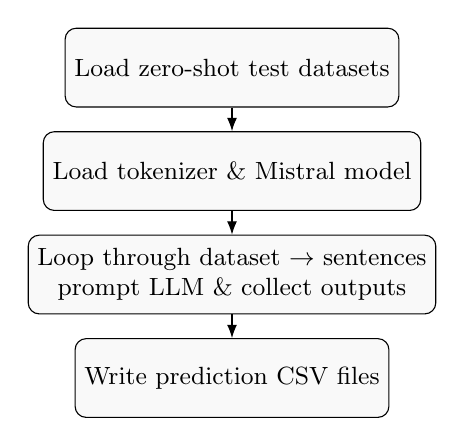
\begin{tikzpicture}[
        node distance=0.3cm,
        every node/.style={font=\small},
        process/.style={rectangle, rounded corners, draw, fill=gray!5, align=center, minimum width=3.6cm, minimum height=1cm},
        line/.style={-Latex}
    ]
        \node[process] (data) {Load zero-shot test datasets};
        \node[process, below=of data] (model) {Load tokenizer \& Mistral model};
        \node[process, below=of model] (loop) {Loop through dataset $\rightarrow$ sentences \\ prompt LLM \& collect outputs};
        \node[process, below=of loop] (csv) {Write prediction CSV files};
        \draw[line] (data) -- (model);
        \draw[line] (model) -- (loop);
        \draw[line] (loop) -- (csv);
    \end{tikzpicture}
    \caption{Zero-shot pipeline for Mistral}
    \label{fig:mistral-zeroshot-pipeline}
\end{figure}

The prompt we used is as follows:

\lstset{
  basicstyle=\ttfamily\small,
  frame=single,
  xleftmargin=2em,
  xrightmargin=2em,
  breaklines=true
}

\begin{lstlisting}
System: You are a linguist who identifies Verlan (French reversed-syllable slang).
Reply with a single digit: '1' if the sentence contains Verlan; otherwise reply '0'.
Do not include extra words.

User: Sentence:
{sentence}

Does this sentence contain Verlan? Reply with one digit (0 or 1).
\end{lstlisting}

For each prompt, we start a new chat session to avoid the influence of the LLM's memorisation\;---\;reusing previous results may interfere with later performance.

A potential issue is that, from time to time, LLMs do not follow the system prompt and produce unexpected responses. The report has accounted for this\;---\;we use regular expressions to extract the numerical values mentioned in the response (i.e., 0 or 1) and store them in a separate column in the CSV file for easier post-processing. We also review the extracted labels manually to prevent inconsistencies or noise.

By doing so, the report believes that the accuracy and reliability of this pipeline are solid.

\subsubsection{Zero-shot of the Most Powerful non deep reasoning LLM as reference}

Considering that both the zero-shot and training experiments above are based on Mistral, the report aims to evaluate performance beyond the Mistral AI ecosystem. After reviewing the \textit{Artificial Analysis Intelligence Index}\footnote{\url{https://artificialanalysis.ai/models/gpt-5-codex\#artificial-analysis-intelligence-index}}, as shown in Figure~\ref{fig:AI_Index}, the report has chosen OpenAI's GPT-5 Codex (High)\footnote{\url{https://openai.com/index/introducing-upgrades-to-codex/}} model as the zero-shot reference. As the top-ranked model, it serves as a strong representative of the current state-of-the-art capabilities in Verlan identification.

\begin{figure}[H]
\centering
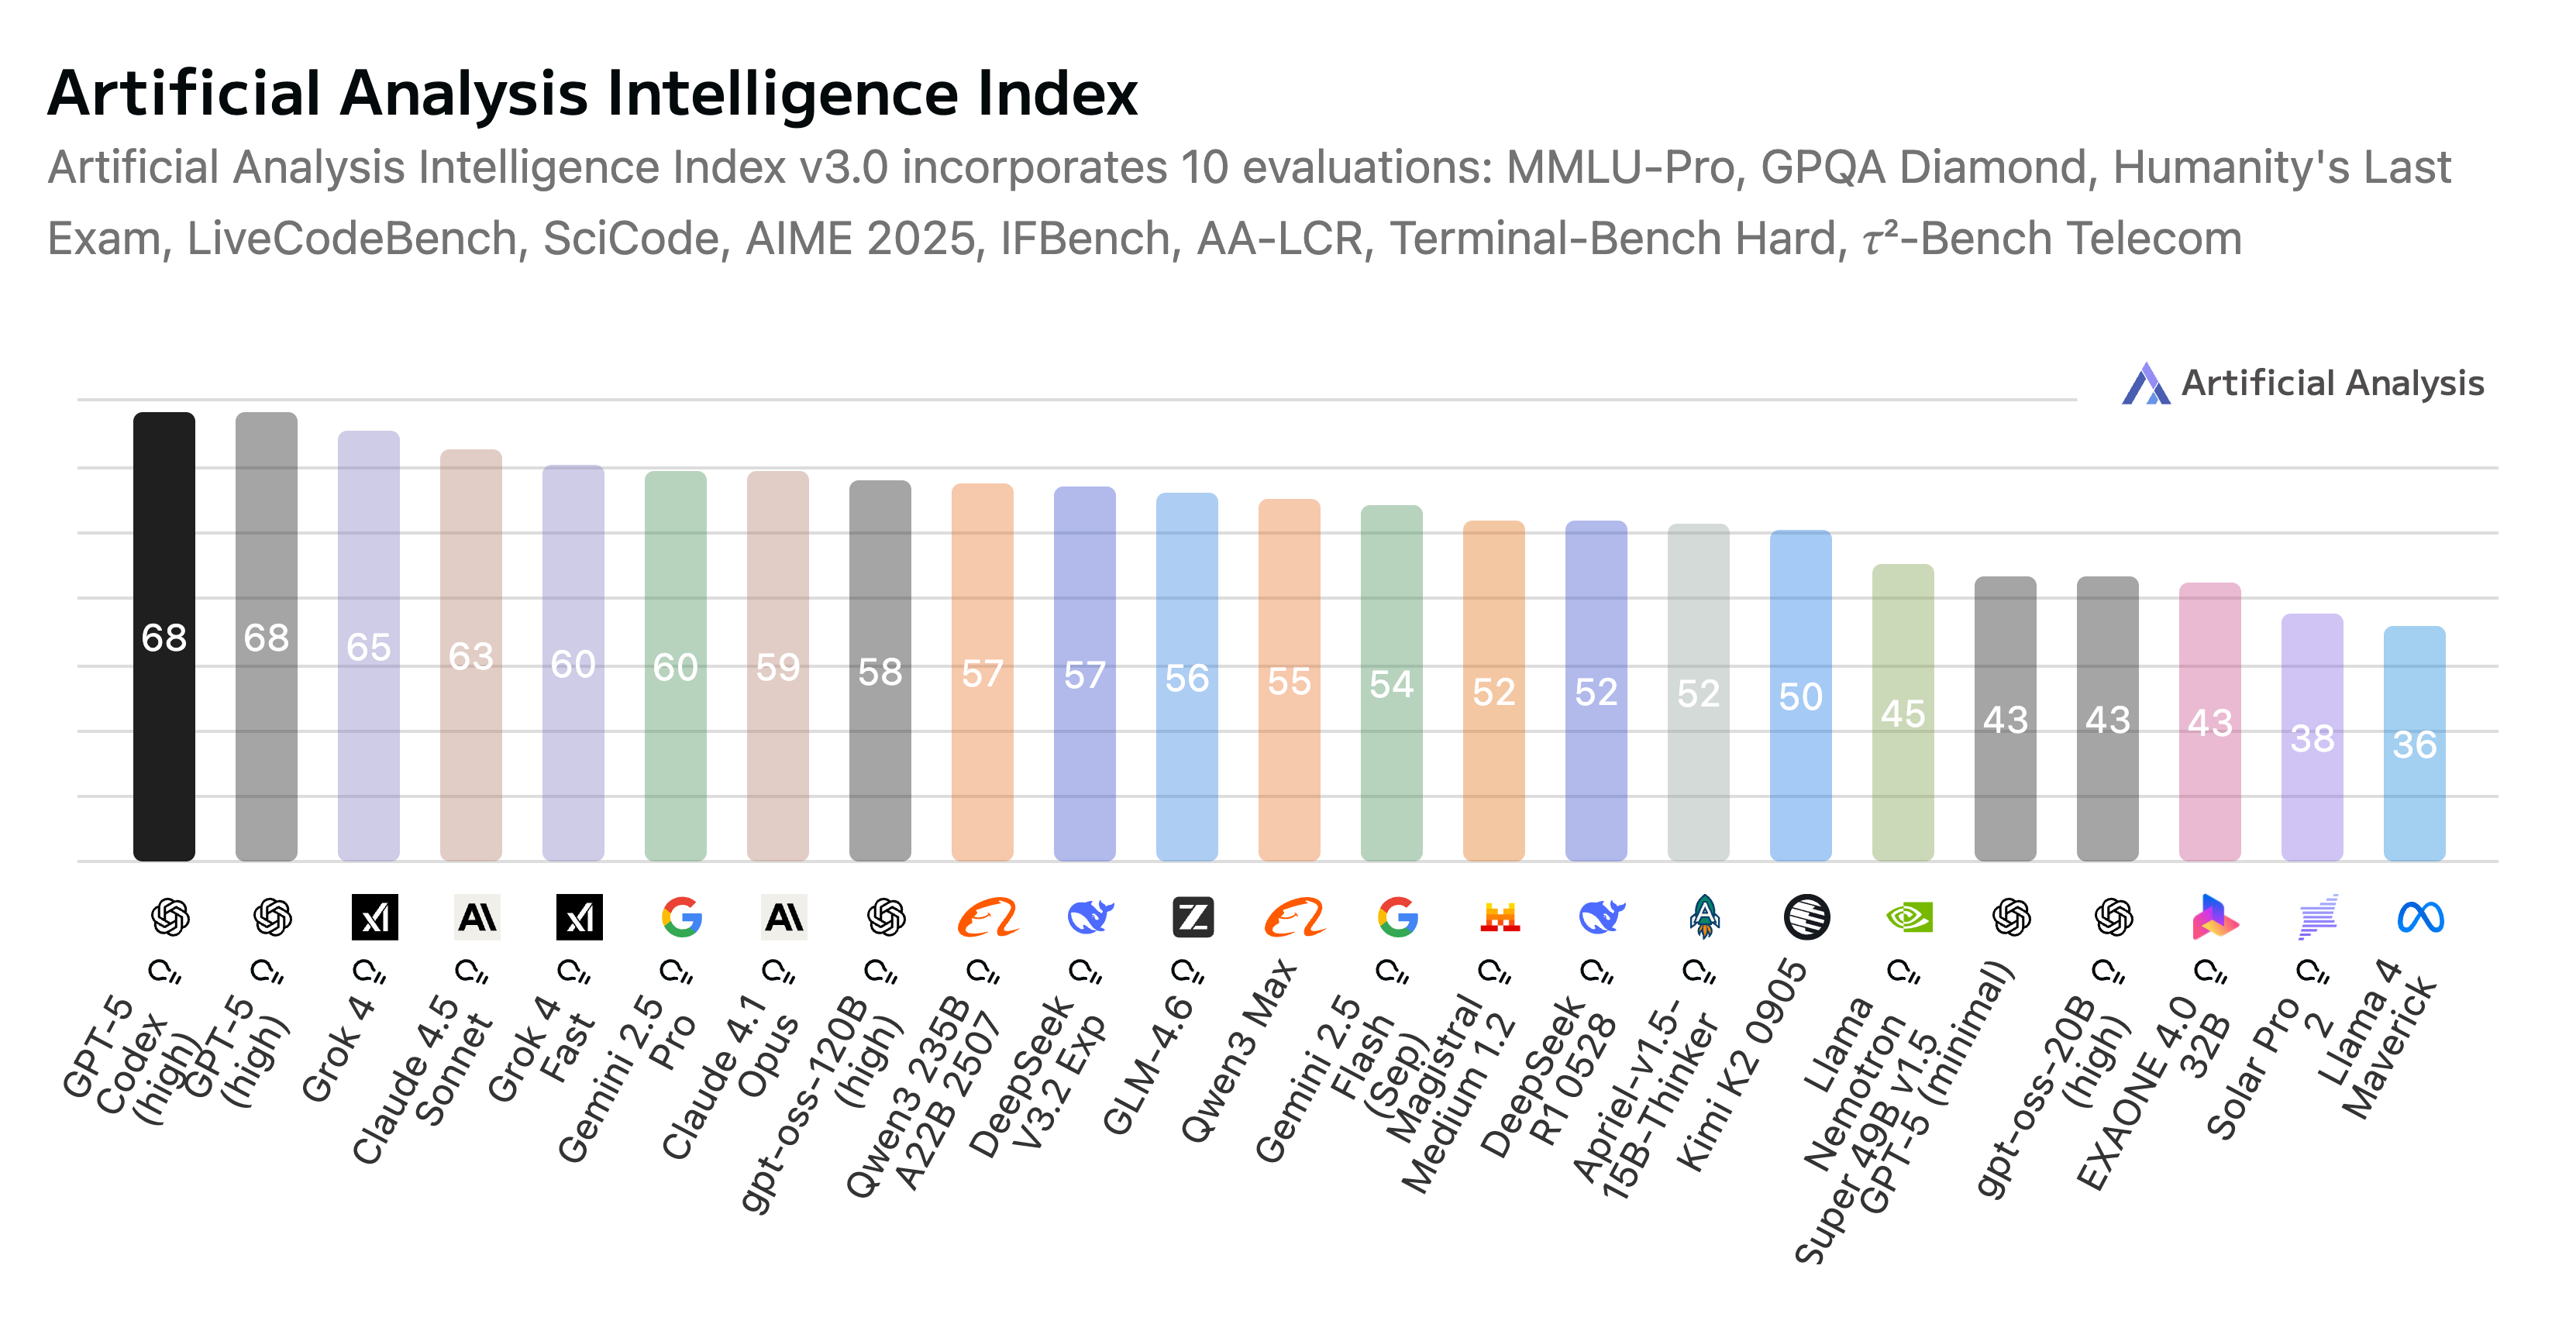
\includegraphics[width=15cm]{figures/Artificial Analysis Intelligence Index (14 Oct '25) .png}
\caption{\label{fig:AI_Index}Leaderboard of the Artificial Analysis Intelligence Index (retrieved on 14 October 2025).}
\end{figure}

Following the principle of controlled experimental design, we used a prompt closely aligned with the one employed for Mistral:

\begin{lstlisting}
[System message]
You are a linguist who identifies verlan (French reversed syllable slang). Ignore any prior memories or cached context and follow only the instructions in this conversation. Do not browse the internet or use external tools; base your reasoning purely on the text you receive here. Reply with a single digit: "1" if the sentence contains verlan; otherwise reply "0". Do not include extra words, punctuation, or explanations.

[User message]
You will be given one or more French sentences. For each sentence, decide whether it contains verlan and answer with a single digit (0 or 1) per sentence, in the same order that the sentences appear.

Sentences to evaluate:
{sentences}
\end{lstlisting}

Notably, because GPT-5 Codex (High) is a reasoning-oriented model, its responses are typically slower, and it also has monthly usage limitations\footnote{The author of this report holds a ChatGPT Plus subscription.}. Therefore, instead of sending each sentence individually with the prompt, we chose to batch all sentences together in a single request. The maximum token size was taken into account, and the total length did not exceed the model's limit of approximately 400,000 tokens.

\subsection{Training Models}
This section introduces the methodology behind the training models. It first explains the pipeline from input to output and how the datasets are split and used within it. Then, it justifies the technical details of the specific hyperparameters and training platforms. Finally, it presents other pipelines that were considered but not implemented in this experiment, along with the rationale behind those decisions.

\subsubsection{The Pipelines}
To avoid confusing readers, the report simplifies the flowcharts to highlight only the key components in this section. The complete flowcharts are provided in the appendix.

\begin{figure}[H]
  \begin{adjustwidth}{-2.0cm}{0cm}
  \centering
  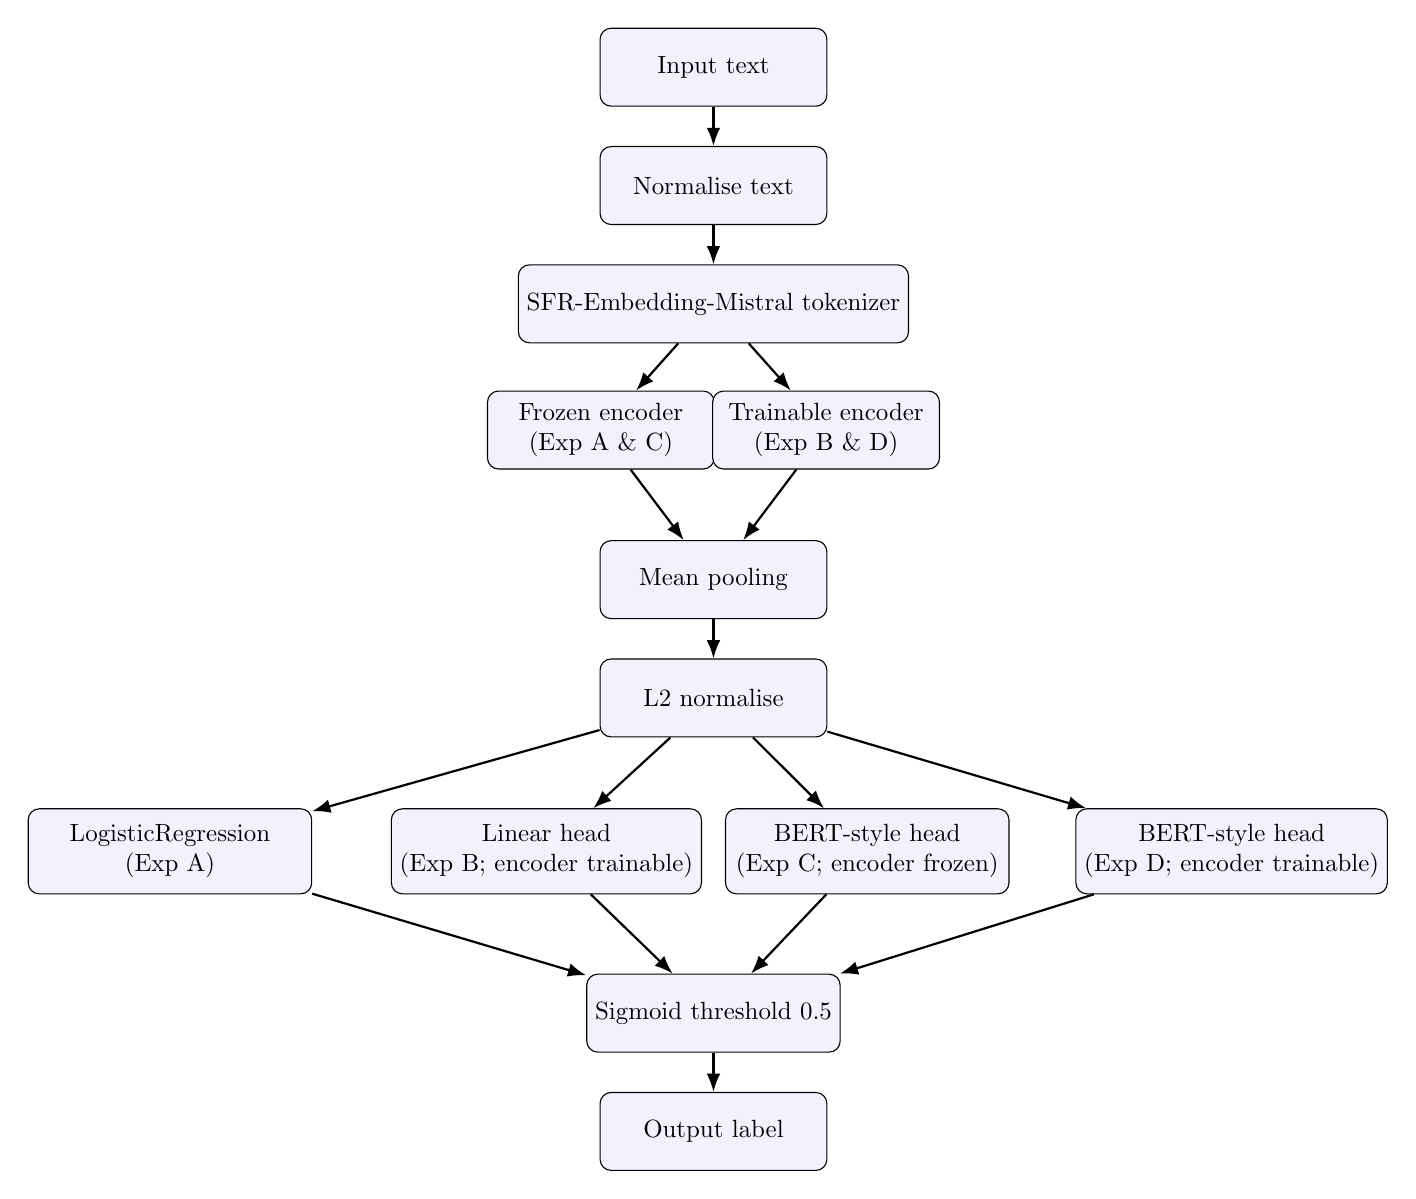
\begin{tikzpicture}[
    >=Latex,
    scale=0.9,
    every node/.style={scale=0.9},
    stage/.style={rectangle, rounded corners, draw=black, fill=blue!5, align=center, minimum width=3.2cm, minimum height=1.1cm},
    head/.style={rectangle, rounded corners, draw=black, fill=blue!5, align=center, minimum width=4.0cm, minimum height=1.2cm},
    node distance=0.5cm,
    font=\normalsize
  ]
    \node[stage] (input) {Input text};
    \node[stage, below=of input] (norm) {Normalise text};
    \node[stage, below=of norm] (tok) {SFR-Embedding-Mistral tokenizer};

    \node[stage, below left=0.6cm and -2.5cm of tok] (encF) {Frozen encoder\\(Exp~A \& C)};
    \node[stage, below right=0.6cm and -2.5cm of tok] (encT) {Trainable encoder\\(Exp~B \& D)};

    \node[stage, below=2.5cm of tok] (mean) {Mean pooling};
    \node[stage, below=of mean] (l2) {L2 normalise};

    \node[head, below left=0.9cm and 3.65cm of l2] (lr) {LogisticRegression\\(Exp~A)};
    \node[head, below left=0.9cm and -1.3cm of l2] (lin) {Linear head\\(Exp~B; encoder trainable)};
    \node[head, below right=0.9cm and -1.3 cm of l2] (bertF) {BERT-style head\\(Exp~C; encoder frozen)};
    \node[head, below right=0.9cm and 3.15cm of l2] (bertT) {BERT-style head\\(Exp~D; encoder trainable)};

    \node[stage, below=3cm of l2] (sig) {Sigmoid threshold 0.5};
    \node[stage, below=of sig] (out) {Output label};

    \draw[->, thick] (input) -- (norm);
    \draw[->, thick] (norm) -- (tok);
    \draw[->, thick] (tok) -- (encF);
    \draw[->, thick] (tok) -- (encT);
    \draw[->, thick] (encF) -- (mean);
    \draw[->, thick] (encT) -- (mean);
    \draw[->, thick] (mean) -- (l2);
    \draw[->, thick] (l2) -- (lr);
    \draw[->, thick] (l2) -- (lin);
    \draw[->, thick] (l2) -- (bertF);
    \draw[->, thick] (l2) -- (bertT);
    \draw[->, thick] (lr) -- (sig);
    \draw[->, thick] (lin) -- (sig);
    \draw[->, thick] (bertF) -- (sig);
    \draw[->, thick] (bertT) -- (sig);
    \draw[->, thick] (sig) -- (out);
  \end{tikzpicture}
  \end{adjustwidth}
  \caption{\label{fig:pipeline-overview}A compact view of the four Verlan identification pipelines.\footnotesize \\Exp~A: Frozen Encoder + LogisticRegression Head\\Exp~B: End-to-End Encoder + Linear Head\\Exp~C: Frozen Encoder + BERT-Style Head\\Exp~D: End-to-End Encoder + BERT-Style Head (Experiment D}
\end{figure}

\paragraph{Input}
The input is the \textit{Sentences} dataset we created. For editing and data management purposes, it is stored as an \texttt{.xlsx} table. It should be noted that the dataset was not converted into a special format before being fed into the pipeline. Therefore, the labels indicating whether a sentence contains a Verlan term remain in the input file when read by the program. However, we are confident that the sentence column was properly isolated, and that no visible data leakage occurred in the program code or during runtime.

\paragraph{Normalise Text}
\subparagraph{Why Not Preserve Upper Cases and Annotation Marks}
As mentioned in Section~3.3.2, we have concerns that the diversity of annotation marks may affect the models' performance. Digging deeper, this is a good argument that even involves thinking about the role of Verlan in a sentence from the LLM's perspective\;---\;a Verlan might be an Out-Of-Vocabulary (OOV) word, or in other words, it might be treated as noise, like typographical mistakes. Indeed, scholars have pointed out that not only typographical mistakes but also annotation marks and the difference between upper and lower cases can all affect model performance\cite{alsharou2021noise}. 

Besides, during a smoke test, the report found that annotation marks and upper/lower case differences can indeed affect model performance. The model mislabels sentences that contain Verlan as if they do not, when the sentence has not been normalised (i.e., trimmed off annotation marks and converted to lowercase). When it has been normalised, the model behaves normally and labels that sentence as containing Verlan.\footnote{Again, it was a non-official test run, so the report cannot claim that we have proven these changes would affect performance. But theoretically, it makes sense that if the LLM treats annotation marks, cases, and Verlan all as noise, normalising the text would reduce unwanted noise and therefore increase accuracy. Further experiments can be conducted if needed.} 

This finding inspired the report to normalise the text before further experiments. Thus, we used regular expressions to trim off the annotation marks and convert the sentences to lowercase, while preserving the rest, including accented letters (e.g., é, à, ù).

\paragraph{Tokenisation}
Because all the encoders used in the four experiments originate from the same Mistral model, it is essential to ensure that the tokens received by the encoder match its expected input format. Therefore, we employ the tokenizer corresponding to Mistral, namely the one developed by Salesforce\;---\;\textit{SFR-Embedding-Mistral}\;---\;to guarantee optimal model performance.

While it is indeed valuable to understand how this tokenizer segments each sentence, this tokenizer-encoder pair already represents the most appropriate configuration for our task. Hence, analysing its internal mechanisms in detail is considered unnecessary for this report.

\paragraph{Encoder}
As mentioned above, the encoders used in these experiments are identical, except that they are run in different modes: frozen or trainable. The reason for comparing a frozen encoder with a trainable one is, firstly, that we believe Verlan identification should be a relatively straightforward task for a large language model (LLM). 

Moreover, given that our dataset contains a limited number of entries, and considering that scholars have pointed out that in many NLP tasks, keeping most of the encoder frozen while fine-tuning only a few layers can still yield strong performance\cite{lodha2023surgical}, a full fine-tuning approach may not be necessary. 

Finally, taking into account both the time required and the expected outcome of partial fine-tuning to find the most optimal ratio between frozen and trainable layers, the report concludes that comparing the two bipolar cases\;---\;fully frozen and fully fine-tuned\;---\;is a more practical and representative approach.

\paragraph{Caliberations}

The report implements caliberations to the last hidden layer of the encoder, specifically, masking, mean pooling and L2 normalisation. 

\subparagraph{Masking}
The implementation of masking can be interpreted as below:

\begin{figure}[H]
\centering
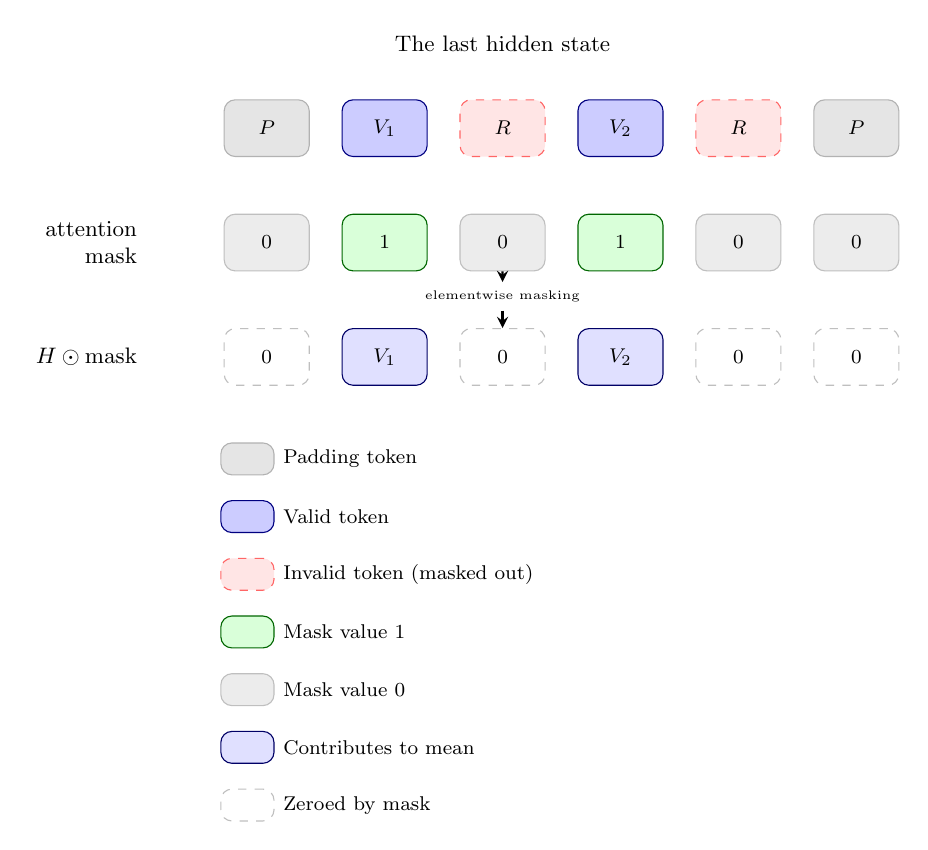
\begin{tikzpicture}[
    scale=0.9,
    every node/.style={transform shape},
    token/.style={rectangle, rounded corners, minimum width=1.2cm, minimum height=0.8cm, font=\footnotesize, align=center},
    valid/.style={token, fill=blue!20, draw=blue!50!black},
    pad/.style={token, fill=gray!20, draw=gray!60},
    removed/.style={token, fill=red!10, draw=red!60, dashed},
    masked/.style={token, fill=blue!12, draw=blue!40!black},
    zeroed/.style={token, fill=white, draw=gray!50, dashed},
    maskone/.style={token, fill=green!15, draw=green!40!black},
    maskzero/.style={token, fill=gray!15, draw=gray!50},
    legend/.style={minimum width=0.75cm, minimum height=0.45cm, inner sep=1.5pt},
    arrow/.style={->, thick, >=stealth}
]

% Row 1: hidden states H = out.last_hidden_state
\node[pad] (h1) {$P$};
\node[valid, right=0.45cm of h1] (h2) {$V_1$};
\node[removed, right=0.45cm of h2] (h3) {$R$};
\node[valid, right=0.45cm of h3] (h4) {$V_2$};
\node[removed, right=0.45cm of h4] (h5) {$R$};
\node[pad, right=0.45cm of h5] (h6) {$P$};
\node[above=0.55cm of h3, font=\small] {The last hidden state};

% Row 2: attention mask (broadcast across hidden size)
\node[maskzero, below=0.8cm of h1] (mask1) {0};
\node[maskone, below=0.8cm of h2] (mask2) {1};
\node[maskzero, below=0.8cm of h3] (mask3) {0};
\node[maskone, below=0.8cm of h4] (mask4) {1};
\node[maskzero, below=0.8cm of h5] (mask5) {0};
\node[maskzero, below=0.8cm of h6] (mask6) {0};
\node[left=1.1cm of mask1, align=right, font=\small] {attention\\mask};

% Row 3: elementwise masked representations (H * mask)
\node[zeroed, below=0.8cm of mask1] (masked1) {0};
\node[masked, below=0.8cm of mask2] (masked2) {$V_1$};
\node[zeroed, below=0.8cm of mask3] (masked3) {0};
\node[masked, below=0.8cm of mask4] (masked4) {$V_2$};
\node[zeroed, below=0.8cm of mask5] (masked5) {0};
\node[zeroed, below=0.8cm of mask6] (masked6) {0};
\node[left=1.1cm of masked1, align=right, font=\small] {$H \odot \text{mask}$};

% Elementwise masking annotation
\node[font=\tiny, align=center, below=0.15cm of mask3] (masknote) {elementwise masking};
\draw[arrow] (mask3.south) -- (masknote.north);
\draw[arrow] (masknote.south) -- (masked3.north);

% ------------------ Legend ------------------
\node[pad, legend, below=0.8cm of masked3, xshift=-3.6cm, label=right:{\footnotesize Padding token}] (legP) {};
\node[valid, legend, below=0.35cm of legP, label=right:{\footnotesize Valid token}] (legV) {};
\node[removed, legend, below=0.35cm of legV, label=right:{\footnotesize Invalid token (masked out)}] (legR) {};
\node[maskone, legend, below=0.35cm of legR, label=right:{\footnotesize Mask value $1$}] (legMone) {};
\node[maskzero, legend, below=0.35cm of legMone, label=right:{\footnotesize Mask value $0$}] (legMzero) {};
\node[masked, legend, below=0.35cm of legMzero, label=right:{\footnotesize Contributes to mean}] (legMasked) {};
\node[zeroed, legend, below=0.35cm of legMasked, label=right:{\footnotesize Zeroed by mask}] (legZeroed) {};

\end{tikzpicture}
\caption{Visulisation of masking.}
\end{figure}

The last hidden state is the final layer of the encoder, where each token has its own hidden representation. 
It has the shape of a three-dimensional tensor, denoted as $\mathbf{H} \in \mathbb{R}^{B \times T \times D}$, 
where $B$ stands for the batch size (the number of sentences in a batch), 
$T$ stands for the sequence length (the number of tokens per sentence), 
and $D$ represents the hidden dimension (the size of each token vector).

Next, we apply the attention mask, which contains $1$s and $0$s. 
A value of $1$ indicates a valid token, while $0$ marks a padding or invalid token that should be ignored. 
However, this mask is \textit{flat}\;---\;it is a two-dimensional tensor, $[B, T]$. 
To ensure it can be broadcast across all $D$ dimensions of each token vector, 
we add an extra dimension at the end of the tensor, resulting in a new shape of $[B, T, 1]$. 
This allows each 0/1 value to be applied consistently across the entire hidden vector of that token.

In the third line of the implementation, the mask is summed along the $T$ dimension, 
yielding the number of valid tokens in each sentence. 
The resulting tensor has the shape $[B, 1]$.

It is always important to handle edge cases. 
If a hidden layer happens to be fully padded, the denominator in the subsequent division could become zero. 
Therefore, we clamp the minimum denominator to $1$ to prevent division-by-zero errors.

\subparagraph{Mean Pooling}
After obtaining the mask, we multiply it with the original hidden state $\mathbf{H}$. 
Here, $\mathbf{H} \in \mathbb{R}^{B \times T \times D}$, while the mask has the shape $[B, T, 1]$. 
By doing so, the mask's last dimension is broadcast to match the $D$ dimension. 
As a result, the $D$-dimensional vectors at valid positions remain unchanged, whereas those at masked (i.e., padding or invalid) positions become zero. 
This operation yields a state with the shape $[B, T, D]$\;---\;the same as the original hidden state, but with masking applied.

Next, we collapse the $T$ dimension by summing all token vectors, resulting in a tensor of shape $[B, D]$. 
We then divide it by the number of valid tokens to obtain the mean representation of the valid tokens. 
The mathematical expression of mean pooling can be formulated as:

\begin{equation}
\text{pooled}[b, :] = 
\frac{\displaystyle \sum_{t=1}^{T} \text{mask}[b, t, 1] \cdot H[b, t, :]}
{\displaystyle \max \!\left( 1, \sum_{t=1}^{T} \text{mask}[b, t, 1] \right)}
\quad \in \mathbb{R}^{D}
\end{equation}

In short, mean pooling computes the average along the $T$ dimension. 
The resulting tensor contains one $D$-dimensional vector per sample in the batch, resulting in the overall shape $[B, D]$.

\subparagraph{L2 Normalisation}
Since we obtain different vectors across the batch, each with potentially varying magnitudes,

\begin{equation}
\mathbf{h}_{\text{pooled}}[b, :] \in \mathbb{R}^{D}
\end{equation}

\noindent their norms can differ. 
However, in the subsequent steps, we care more about the \textit{direction} rather than the magnitude of these vectors. 
Therefore, we apply L2 normalisation to project all vectors onto the unit hypersphere, unifying their magnitudes to $1$:

\begin{equation}
\|\mathbf{h}_{\text{norm}}[b, :]\|_2 = 1
\end{equation}

\noindent The normalised vectors are computed as:

\begin{equation}
\mathbf{h}_{\text{norm}}[b, :] =
\frac{\mathbf{h}_{\text{pooled}}[b, :]}
{\|\mathbf{h}_{\text{pooled}}[b, :]\|_2 + \epsilon}
\quad \in \mathbb{R}^{D}
\end{equation}

\noindent where the L2 norm is defined as:

\begin{equation}
\|\mathbf{h}_{\text{pooled}}[b, :]\|_2
= \sqrt{\sum_{i=1}^{D} \left(\mathbf{h}_{\text{pooled}}[b, i]\right)^2},
\end{equation}

\noindent and $\epsilon$ is a small constant added to prevent division by zero.

By applying L2 normalisation, we ensure that the similarity between samples depends solely on the angular difference between their directions, which leads to more stable and comparable representations.

\paragraph{The Classifiers\;---\;Logistic Regression or BERT}
The primary difference among the four experiments lies here\;---\;not only in the choice between Logistic Regression and BERT, but also in the implementation framework, namely scikit-learn versus PyTorch.

\subparagraph{Logistic Regression with scikit-learn}
For the experiment using a frozen encoder with a \textit{Logistic Regression} head, we chose to employ scikit-learn (sklearn)\footnote{\url{https://scikit-learn.org}}. 
It is simple to implement, and its \texttt{LogisticRegression} function internally handles both the loss computation and the optimiser. 
In contrast, the other three experiments involve learning and therefore use PyTorch\footnote{\url{https://pytorch.org/}} instead. 
Unlike scikit-learn, PyTorch does not provide built-in loss or optimiser functions for such cases, so these components are implemented explicitly, as illustrated in Figure~8. 
For the latter three experiments, both BERT and Logistic Regression (the linear layer) act as \textit{heads}, whereas this experiment is referred to simply as \textit{Logistic Regression}.

\subparagraph{BERT-Style Head}
Regardless of whether it is Logistic Regression or BERT, both function as the classifier component\;---\;they process the normalised sentence vectors to determine whether a sentence contains Verlan or not. 
Logistic Regression is merely a linear classifier; it cannot learn potential semantic patterns in the same way as the Mistral encoder. 
As mentioned earlier, CamemBERT serves as an alternative LLM to Mistral in this experiment. 
To combine the advantages of both and maximise their potential, we therefore employ BERT as another type of classifier.

However, BERT itself, much like the zero-shot Mistral tested earlier, is a complete LLM\;---\;it contains all the essential components such as a tokenizer, an encoder, and a classifier. 
Thus, it would be impractical to connect an entire BERT model after the Mistral encoder, as this would result in a redundant pipeline: Mistral embedder, Mistral tokenizer, Mistral encoder, BERT tokenizer, BERT encoder, BERT classifier, and so on. 
Therefore, we only utilise the \textit{classifier head} from BERT.

%classical BERT
\begin{figure}[H]
\centering
\begin{adjustwidth}{-0.3cm}{0cm}
\begin{minipage}{1\textwidth}
\centering
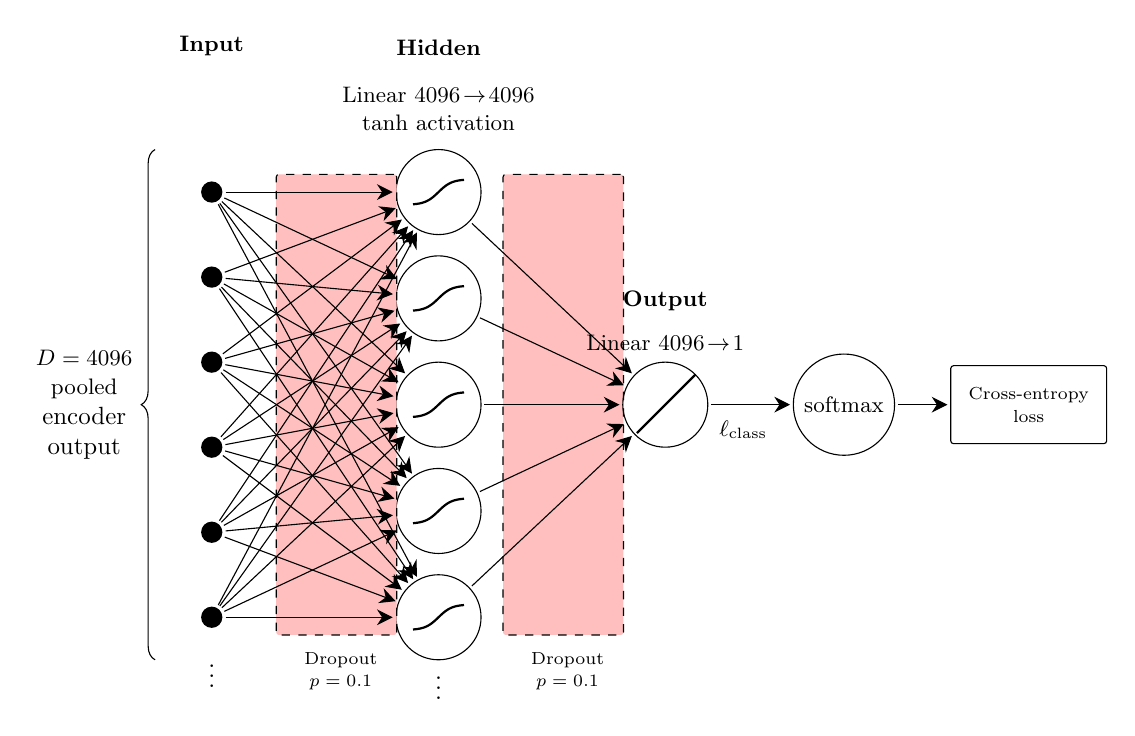
\begin{tikzpicture}[node distance=16mm and 22mm, scale=0.9, every node/.style={transform shape}]

% Column anchors
\coordinate (C0) at (0,0);      % pooled input
\coordinate (C1) at (3.2,0);    % hidden tanh
\coordinate (C2) at (6.4,0);    % output logit

% ===== Pooled encoder representation =====
\foreach [count=\i] \y in {30mm,18mm,6mm,-6mm,-18mm,-30mm} {
  \node[inDot] (x\i) at ($(C0)+(0,\y)$) {};
}
\draw[decorate,decoration={brace,mirror,amplitude=5pt}]
  ($(x1)+(-8mm,6mm)$) -- ($(x6)+(-8mm,-6mm)$)
  node[midway,xshift=-10mm,align=center] {\small $D=4096$\\\small pooled\\encoder\\output};
\node at ($(x1)!1.4!(x5)$) {$\vdots$};
\node[layerlabel] at ($(x1)+(0,18mm)$) {\textbf{Input}};

% ===== Hidden (tanh) layer =====
\foreach [count=\i] \y in {30mm,15mm,0mm,-15mm,-30mm} {
  \node[tanhNeuron] (h\i) at ($(C1)+(0,\y)$) {};
}
\node at ($(h1)!1.15!(h5)$) {$\vdots$};
\node[layerlabel] at ($(h1)+(0,18mm)$) {\textbf{Hidden}};
\node[anchor=north, font=\small, align=center] at ($(h1)+(0,16mm)$) {Linear $4096\!\rightarrow\!4096$\\$\tanh$ activation};

% ===== Dropout annotations =====
\node[draw, dashed, rounded corners=1pt, fill=pink, minimum width=17mm, minimum height=65mm]
  (dropBeforeCls) at ($(C0)!0.55!(C1)$) {};
\node[font=\scriptsize, align=center, anchor=east]
  at ($(dropBeforeCls.south)+(7mm,-5mm)$) {\shortstack{Dropout\\$p=0.1$}};
\node[draw, dashed, rounded corners=1pt, font=\scriptsize, fill=pink, minimum width=17mm, minimum height=65mm]
  (dropBetweenCls) at ($(C1)!0.55!(C2)$) {};
\node[font=\scriptsize, align=center, anchor=east]
  at ($(dropBetweenCls.south)+(7mm,-5mm)$)  {\shortstack{Dropout\\$p=0.1$}};

% ===== Output (logit) =====
\node[linearNeuron] (o1) at ($(C2)+(0,0mm)$) {};
\node[layerlabel, anchor=south] at ($(o1.south)+(11mm,0mm)$) {$\ell_{\text{class}}$};
\node[layerlabel] at ($(o1)+(0,12mm)$) {\textbf{Output}};
\node[anchor=north, font=\small, align=center] at ($(o1)+(0,11mm)$) {Linear $4096\!\rightarrow\!1$};

% ===== Connections (fully connected) =====
\foreach \a in {1,...,6} {\foreach \b in {1,...,5} {\draw[->,shorten >=1pt,shorten <=1pt] (x\a) -- (h\b);}}
\foreach \a in {1,...,5} {\draw[->,shorten >=1pt,shorten <=1pt] (h\a) -- (o1);};

% ===== Softmax + loss =====
\node[draw, circle, minimum size=11mm, font=\small, anchor=west] (softmaxClass) at ($(o1)+(18mm,0)$) {$\mathrm{softmax}$};
\draw[->,shorten >=1pt,shorten <=1pt] (o1.east) -- (softmaxClass.west);
\node[draw, rounded corners=1pt, minimum width=22mm, minimum height=11mm, font=\scriptsize, anchor=west]
  (lossClass) at ($(softmaxClass)+(15mm,0)$) {\shortstack{Cross-entropy\\loss}};
\draw[->,shorten >=1pt,shorten <=1pt] (softmaxClass.east) -- (lossClass.west);

\end{tikzpicture}
\end{minipage}
\end{adjustwidth}
\caption{Classic BERT classification head.}
\label{fig:bert-classification-head}
% --- END CLASSIFICATION HEAD FIGURE ---
\end{figure}

Figure~10 illustrates the internal structure of a standard BERT classifier. 
It receives the pooled output from the encoder with a dimensionality of 4096, then applies dropout\;---\;randomly setting 10\% of the neurons to zero to prevent overfitting. 
Since the neurons are linear, they are subsequently transformed with a \texttt{tanh} activation for improved non-linearity within the hidden layer. 
After that, dropout is applied again before mapping the 4096 hidden neurons to a single linear output neuron. 
Finally, a softmax function converts the output into a probability distribution, which is then passed to the cross-entropy loss for evaluation.

However, because we are performing model fusion\;---\;that is, blending layers from two different LLMs\;---\;certain adaptations are required:

\begin{enumerate}
  \item We have not only applied mean pooling but also normalisation to the output of the Mistral encoder. 
  While the original BERT classifier uses only pooled features, we include normalisation to maximise fusion performance.
  \item In the classic BERT classifier, the output logit is followed by a softmax function and a loss calibration step. 
  In our case, we require a binary output (0 or 1), so we adopt a different loss function, calibration method, and thresholding strategy to produce binary results consistent with the design of the \textit{Logistic Regression with scikit-learn} experiment.
\end{enumerate}

%BERT-style
\begin{figure}[H]
\centering
\begin{minipage}{1\textwidth}
\begin{adjustwidth}{-2.5cm}{0cm} % shift entire figure 1cm to the left
\centering
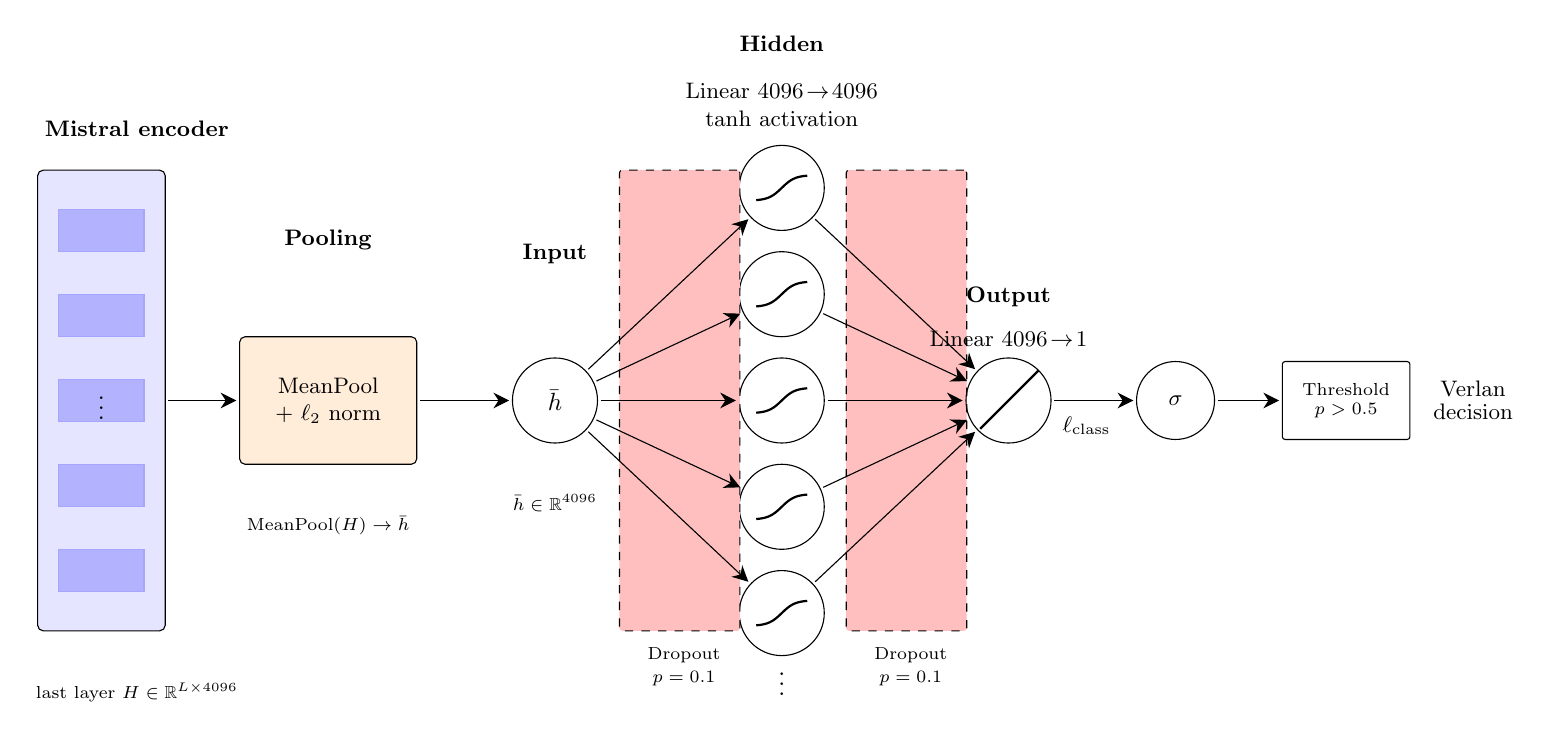
\begin{tikzpicture}[node distance=16mm and 22mm, scale=0.9, every node/.style={transform shape}]

% Column anchors
\coordinate (Cminus2) at (-6.4,0); % Mistral encoder output
\coordinate (Cminus1) at (-3.2,0); % pooling + normalisation
\coordinate (C0) at (0,0);        % pooled vector
\coordinate (C1) at (3.2,0);      % hidden tanh
\coordinate (C2) at (6.4,0);      % output logit

% ===== Mistral encoder outputs =====
\node[draw, rounded corners=2pt, fill=blue!10, minimum width=18mm, minimum height=65mm] (mistralLast) at (Cminus2) {};
\foreach \y in {24mm,12mm,0mm,-12mm,-24mm} {
  \node[rectangle, draw=blue!35, fill=blue!30, minimum width=12mm, minimum height=6mm] at ($(mistralLast.center)+(0,\y)$) {};
}
\node at ($(mistralLast.north)!0.5!(mistralLast.south)$) {$\vdots$};
\node[layerlabel] at ($(mistralLast)+(5mm,36mm)$) {\textbf{Mistral encoder}};
\node[font=\scriptsize, align=center, anchor=north] at ($(mistralLast.south)+(5mm,-6mm)$) {last layer $H \in \mathbb{R}^{L \times 4096}$};

% ===== Mean pooling + normalisation =====
\node[draw, rounded corners=2pt, fill=orange!15, minimum width=25mm, minimum height=18mm, font=\small, align=center] (meanPool) at (Cminus1) {\text{MeanPool}\\$+\ \ell_2$ norm};
\node[layerlabel] at ($(meanPool)+(0,20mm)$) {\textbf{Pooling}};
\node[font=\scriptsize, align=center, anchor=north] at ($(meanPool.south)+(0,-6mm)$) {$\text{MeanPool}(H) \rightarrow \bar{h}$};
\draw[->,shorten >=1pt,shorten <=1pt] (mistralLast.east) -- (meanPool.west);

% ===== Pooled representation =====
\node[neuron] (hbar) at (C0) {$\bar{h}$};
\node[layerlabel] at ($(hbar)+(0,18mm)$) {\textbf{Input}};
\node[font=\scriptsize, align=center, anchor=north] at ($(hbar.south)+(0,-6mm)$) {$\bar{h} \in \mathbb{R}^{4096}$};
\draw[->,shorten >=1pt,shorten <=1pt] (meanPool.east) -- (hbar.west);

% ===== Hidden (5 tanh; represent 4096) =====
\foreach [count=\i] \y in {30mm,15mm,0mm,-15mm,-30mm} {
  \node[tanhNeuron] (h\i) at ($(C1)+(0,\y)$) {};
}
\node at ($(h1)!1.15!(h5)$) {$\vdots$};
\node[layerlabel] at ($(h1)+(0,18mm)$) {\textbf{Hidden}};
\node[anchor=north, font=\small, align=center] at ($(h1)+(0,16mm)$) {Linear $4096\!\rightarrow\!4096$\\$\tanh$ activation};

% ===== Dropout annotations =====
\node[draw, dashed, rounded corners=1pt, fill=pink, minimum width=17mm, minimum height=65mm]
  (dropBefore) at ($(C0)!0.55!(C1)$) {};
\node[font=\scriptsize, align=center, anchor=east]
  at ($(dropBefore.south)+(7mm,-5mm)$) {\shortstack{Dropout\\$p=0.1$}};
\node[draw, dashed, rounded corners=1pt, fill=pink, minimum width=17mm, minimum height=65mm]
  (dropBetween) at ($(C1)!0.55!(C2)$) {};
\node[font=\scriptsize, align=center, anchor=east]
  at ($(dropBetween.south)+(7mm,-5mm)$) {\shortstack{Dropout\\$p=0.1$}};

  % ===== Output (single logit) =====
\node[linearNeuron] (o1) at ($(C2)+(0,0mm)$) {};
\node[layerlabel, anchor=south] at ($(o1.south)+(11mm,0mm)$) {$\ell_{\text{class}}$};
\node[layerlabel] at ($(o1)+(0,12mm)$) {\textbf{Output}};
\node[anchor=north, font=\small, align=center] at ($(o1)+(0,11mm)$) {Linear $4096\!\rightarrow\!1$};

% ===== Connections (fully connected) =====
\foreach \b in {1,...,5} {\draw[->,shorten >=1pt,shorten <=1pt] (hbar) -- (h\b); }
\foreach \a in {1,...,5} {\draw[->,shorten >=1pt,shorten <=1pt] (h\a) -- (o1);};

% ===== Sigmoid + threshold gate =====
\node[draw, circle, minimum size=11mm, font=\small, anchor=west] (sigmoidDetect) at ($(o1)+(18mm,0)$) {$\sigma$};
\draw[->,shorten >=1pt,shorten <=1pt] (o1.east) -- (sigmoidDetect.west);
\node[draw, rounded corners=1pt, minimum width=18mm, minimum height=11mm, font=\scriptsize, anchor=west]
  (thresholdDetect) at ($(sigmoidDetect)+(15mm,0)$) {\shortstack{Threshold\\$p>0.5$}};
\draw[->,shorten >=1pt,shorten <=1pt] (sigmoidDetect.east) -- (thresholdDetect.west);
\node[anchor=west, font=\small] at ($(thresholdDetect.east)+(2mm,0)$) {\shortstack{Verlan\\decision}};

\end{tikzpicture}
\end{adjustwidth}
\end{minipage}
\caption{BERT-style detection head.}
\label{fig:bert-detect-head}
% --- END DETECTION HEAD FIGURE ---
\end{figure}

As shown in Figure~11, we modify the standard BERT classifier accordingly. 
We continue to refer to it as \textit{BERT}, but use the term \textit{BERT-style} to emphasise that structural adjustments have been made for model fusion optimisation.

\subparagraph{The Different Loss Function and Calibration}

As mentioned above, after the linear output neuron, we use a different loss function\;---\;\texttt{BCEWithLogitsLoss}\;---\;and a calibrator, AdamW\cite{paszke2019pytorch,loshchilov2019adamw}.

The \textit{Binary Cross-Entropy (BCE)} loss is used in binary classification tasks. It measures the cross-entropy between the predicted probability distribution and the true label:
\begin{equation}
\mathcal{L}_{\mathrm{BCE}}(y, \hat{y}) = - \big[ y \cdot \log(\hat{y}) + (1 - y) \cdot \log(1 - \hat{y}) \big]
\end{equation}
where
\begin{equation}
y \in \{0, 1\}, \quad \hat{y} = \sigma(z) = \frac{1}{1 + e^{-z}}
\end{equation}

According to the formula, the essence of BCE is to minimise the cross-entropy between the predicted distribution and the true distribution.

The \texttt{BCEWithLogitsLoss} function in PyTorch applies the sigmoid operation to the logits internally and then computes the BCE loss. Its numerically stable formulation is:
\begin{equation}
\mathcal{L}_{\mathrm{BCEWithLogits}}(y, z) = \max(z, 0) - z \cdot y + \log\big(1 + e^{-|z|}\big)
\end{equation}

This formulation prevents numerical underflow or overflow when the model becomes overconfident\;---\;that is, when the logit $z$ is very large or very small. In such cases, a direct computation of BCE might yield $0$ or $\infty$, causing the training to crash or the gradient to become \texttt{NaN}. Hence, \texttt{BCEWithLogitsLoss} is more numerically stable than the pure BCE function.

\textit{Adaptive Moment Estimation (Adam)} is a self-adaptive learning rate optimisation algorithm\cite{kingma2014adam}. It elegantly integrates concepts from mathematics, physics, and computer science\;---\;it is based on the idea of momentum\footnote{\url{https://en.wikipedia.org/wiki/Momentum}} and takes into account both the first-order moment (the mean of gradients) and the second-order moment (the uncentred variance of gradients).

For each iteration $t$, given the gradient $g_t = \nabla_\theta \mathcal{L}(\theta_t)$,  
the Adam update rules are defined as follows:
\begin{equation}
\begin{aligned}
m_t &= \beta_1 \, m_{t-1} + (1 - \beta_1) \, g_t \\
v_t &= \beta_2 \, v_{t-1} + (1 - \beta_2) \, g_t^2 \\
\hat{m}_t &= \frac{m_t}{1 - \beta_1^t} \\
\hat{v}_t &= \frac{v_t}{1 - \beta_2^t} \\
\theta_{t+1} &= \theta_t - \alpha \, \frac{\hat{m}_t}{\sqrt{\hat{v}_t} + \epsilon}
\end{aligned}
\end{equation}

where:
\begin{itemize}
    \item $\beta_1, \beta_2$ are the exponential decay rates for the first and second moment estimates (commonly 0.9 and 0.999);
    \item $\epsilon$ is a small constant for numerical stability;
    \item $\alpha$ is the learning rate;
    \item $m_t$ is the first moment estimate;
    \item $v_t$ is the second moment estimate.
\end{itemize}

\textit{Adam with Decoupled Weight Decay (AdamW)} further improves the optimisation process by decoupling the weight decay from the gradient update, thus correcting the regularisation deficiency in Adam\cite{loshchilov2019adamw}:
\begin{equation}
\begin{aligned}
m_t &= \beta_1 \, m_{t-1} + (1 - \beta_1) \, g_t \\
v_t &= \beta_2 \, v_{t-1} + (1 - \beta_2) \, g_t^2 \\
\hat{m}_t &= \frac{m_t}{1 - \beta_1^t}, \quad
\hat{v}_t = \frac{v_t}{1 - \beta_2^t} \\
\theta_{t+1} &= \theta_t - \alpha \left( \frac{\hat{m}_t}{\sqrt{\hat{v}_t} + \epsilon} + \lambda \theta_t \right)
\end{aligned}
\end{equation}

where $\lambda$ is the weight decay coefficient.  
Unlike Adam, AdamW does not add the L2 regularisation term directly to the loss function; instead, it applies the decay explicitly to the weights. This modification ensures a consistent regularisation effect and often leads to better generalisation performance.

By applying these two techniques\;---\;a numerically stable loss function and a decoupled regularisation optimiser\;---\;the model is expected to achieve improved convergence stability and higher predictive accuracy.

\paragraph{The Sigmoid Threshold}
%Threshold = fixed, 0.5

\subsubsection{The Usage of the Datasets}
%how I split the dataset into train, validation and test
%where and when to feed them into the pipeline

\subsubsection{Environment and Hyperparameters}
%all the experiments have been conducted on the Aoraki computing cluster of the University of Otago, Otakou whakaihu Waka.
% all used Nvidia L40
%All 4-bit quantised
%etc

\subsection{Other Models}
\subsubsection{Justifying for LR}
% I'm not connecting LR head directly, if so, I've tested, I got NO separation.
\subsubsection{Calibration: Temp / Platt / Isotonic / Threshold Tuning}
%tested these, but to simplify the pipeline, we decided to use 0.5 hard limitation instead
\subsubsection{Gazetteer Gate}
% using the dictionary dataset for this. Not using this in real experiment because it is too powerful and causing overfitting-like issues

%%%%%%%%%%%%%%%%%%%%%%%%%%%%%%%%%%%%%%%%%%%%%%%%%%%%%%%%%%%%%%%%%%%%%%%%%%%%%%%%%%%%%%%%%%%%%%%%%%%%%%%%%%%%%%%%%%%%%%%%%%%%%%%%%%%%%%%%%%%%%%%%%%%%%%%%%%%%%%%%%%%%%%%%%%%%%%%%%%%%%%%%%%%%%%%%%%%%%%%%%%%%%%%%%%%%%%%%%%%%%%%%%%%%%%%%%%%%%%%%%%%%%%%%%%%%
\section{Experiments, Results, and Analyses}
%mention again, the experiments are run on Aoraki.

%Embedding or Encoder; for embedding, need to show embedding space figures 
\subsection{Evaluation Methodology}
\subsubsection{Testing Datasets}
%justify the testing dataset here is not the testing part in the training dataset
%mixed modern verlans, invented verlans, slangs
% especially explain why we need to test slangs
\subsubsection{Testing Schema}
% for zero-shot models, we only evaluated them based on the testing dataset, not the training dataset --- not necessary.
%trained each case's model 20 times and tested 20 times with different seeds to reduce bias

\subsection{Results}
\textbf{Draft note.} Tables~\ref{tab:main-test-confusion-draft} and~\ref{tab:aux-test-confusion-draft} sketch the raw confusion counts gathered from the six shortlisted systems.  The learned verlan detectors (especially the end-to-end BERT variant) reach the best overall balance on the main held-out split, whereas both zero-shot models remain brittle on slang and invented verlan.  Invented forms are the hardest slice for every model, with even the strongest system missing more than half of the positives.



\begin{table}[H]
    \centering
    \footnotesize
    \begin{tabular}{lrrrrrr}
        \hline
        Model & \multicolumn{2}{c}{Existed verlan (TP/FN)} & \multicolumn{2}{c}{Invented verlan (TP/FN)} & \multicolumn{2}{c}{French slang (TN/FP)} \\
         & TP & FN & TP & FN & TN & FP \\
        \hline
        Frozen+LR & 20 & 9 & 8 & 17 & 18 & 7 \\
        E2E+LR & 19 & 10 & 6 & 19 & 16 & 9 \\
        Frozen+BERT & 24 & 5 & 12 & 13 & 20 & 5 \\
        E2E+BERT & 19 & 10 & 4 & 21 & 19 & 6 \\
        Mistral-7B Zero Shot & 22 & 7 & 17 & 8 & 11 & 14 \\
        ChatGPT 5 Thinking Zero Shot & 23 & 6 & 23 & 2 & 20 & 5 \\
        \hline
    \end{tabular}
    \caption{Draft confusion-count summary on the auxiliary targeted suites: curated historical verlan pairs (29 samples), self-created verlan forms (25 samples), and contemporary slang paraphrases (25 samples).  Only verlan variants are shown for the verlan suites, so TN/FP are omitted there.  ChatGPT operates on 158 prompt responses in total across both tables.}
    \label{tab:aux-test-confusion-draft}
\end{table}

\subsection{Analyses}
\subsubsection{Zero-Shot Mistral-7B Model}
\subsubsection{Frozen Encoder + LogisticRegression Head (Experiment A)}
%we write this in detail, explaining everything we have in the pipeline
\subsubsection{Frozen Encoder + BERT-Style Head (Experiment C)}
%less detail
\subsubsection{End-to-End Encoder + Linear Head (Experiment B)}
%more detail on the E2E process
\subsubsection{End-to-End Encoder + BERT-Style Head (Experiment D)}
\subsubsection{Zero-Shot ChatGPT 5 Codex (High)}


\subsection{Conclusion and Limitation}

\section{Discussion and Outlook}
% for Mistral zero shot, shoulda run under different temps

% Besides, identifying the same word with different spelling or declensions is also a hurdle. although we do have those fuzzy search algorithms, the report is not sure whether 

\newpage
%TC:ignore
\begin{thebibliography}{9}

\bibitem{rajabov2025} 
Radjabov, Ruslan Rajabmurodovich. \textit{Understanding "verlan" in the French Language}. 
Web of Scientist: International Scientific Research Journal, vol. 6, no. 3, 2025, pp. 368-372. 
Available at: \url{https://webofjournals.com/index.php/3/article/view/3264}.

\bibitem{bach2018} 
Bach, Xavier. \textit{Tracing the origins of verlan in an early nineteenth century text}. 
Journal of French Language Studies, vol. 28, no. 1, 2018, pp. 1-18. 
Cambridge University Press. doi:10.1017/S0959269516000221.

\bibitem{evolutionverlan} 
Olivier Sécardin. \textit{Évolution du verlan, marqueur social et identitaire, comme reflet de la langue et de la société françaises}. 
Synergies Europe, no. 3, 2008, pp. 223-232. 
Available at: \url{https://journal.lib.uoguelph.ca/index.php/synergies/article/download/1037/1859?inline=1}.

\bibitem{rua2005} 
Rúa, Paula López. “Shortening Devices in Text Messaging.” 
\textit{Journal of Computer-Mediated Communication}, vol. 10, no. 4, July 2005. 
Wiley. doi:10.1111/j.1083-6101.2005.tb00268.x.

\bibitem{hajiyeva2025}  
Hajiyeva, Bulbul. “Translating Idioms and Slang: Problems, Strategies, and Cultural Implications.”  
Acta Globalis Humanitatis et Linguarum, vol. 2, no. 2, 2025, pp. 284-293. doi:10.69760/aghel.025002123.  

\bibitem{deepl2020} 
DeepL. “DeepL Translator translates texts using artificial neural networks. These networks are trained on many millions of translated texts.” 
\textit{DeepL Blog}, 2020. Available at: \url{https://www.deepl.com/en/blog/how-does-deepl-work}.

\bibitem{wu2016} 
Wu, Yonghui, et al. “Google's Neural Machine Translation System: Bridging the Gap between Human and Machine Translation.” 
arXiv preprint arXiv:1609.08144, 2016. Available at: \url{https://arxiv.org/abs/1609.08144}.

\bibitem{michel2018mtnt}
Michel, Paul, and Graham Neubig. “MTNT: A Testbed for Machine Translation of Noisy Text.”
\textit{Proceedings of EMNLP}, 2018. Available at: \url{https://aclanthology.org/D18-1050/}.

\bibitem{zurbuchen2024}
Zurbuchen, Lucas, and Rob Voigt.  
\textit{A Computational Analysis and Exploration of Linguistic Borrowings in French Rap Lyrics}.  
In *Proceedings of the 62nd Annual Meeting of the Association for Computational Linguistics — Student Research Workshop (ACL SRW 2024)*, 2024, pp. 200-208.  
DOI: 10.18653/v1/2024.acl-srw.27.  

\bibitem{podhorna2020rapcor}
Podhorná-Polická, Alena.  
\textit{RapCor, Francophone Rap Songs Text Corpus}.  
In *Proceedings of the Fourteenth Workshop on Recent Advances in Slavonic Natural Language Processing (RASLAN 2020)*, 2020, pp. 95-102.  
Available at: \url{https://nlp.fi.muni.cz/raslan/raslan20.pdf#page=95}.  % (no DOI found)

\bibitem{mekki2021tremolo}
Mekki, Jade; Lecorvé, Gwénolé; Battistelli, Delphine; Béchet, Nicolas.  
\textit{TREMoLo-Tweets: A Multi-Label Corpus of French Tweets for Language Register Characterization}.  
In *Proceedings of the International Conference on Recent Advances in Natural Language Processing (RANLP 2021)*, Held Online, INCOMA Ltd., Sep 1-3, 2021, pp. 950-958.  
DOI: 10.26615/978-954-452-072-4\_108.  

\bibitem{panckhurst202088milsms}
Panckhurst, Rachel; Lopez, Cédric; Roche, Mathieu.  
\textit{A French text-message corpus: 88milSMS. Synthesis and usage}.  
Corpus [En ligne], 20 | 2020 (mis en ligne le 28 janvier 2020).  
DOI: 10.4000/corpus.4852.  

\bibitem{pei2019slang}
Pei, Zhengqi, Zhewei Sun, and Yang Xu.  
\textit{Slang Detection and Identification}.  
In *Proceedings of the 23rd Conference on Computational Natural Language Learning (CoNLL 2019)*, Hong Kong, China, 2019, pp. 881-889.  
Available at: \url{https://aclanthology.org/K19-1082/}.  % (ACL Anthology entry — no DOI)

\bibitem{sun2024informal}
Sun, Zhewei, Qian Hu, et al.  
\textit{Toward Informal Language Processing: Knowledge of Slang in Large Language Models}.  
In *Proceedings of the 2024 Conference of the North American Chapter of the Association for Computational Linguistics (NAACL 2024)*, 2024.  
DOI: 10.18653/v1/2024.naacl-long.94.  

\bibitem{slangornot2024}
Anonymous.  
\textit{Slang or Not? Exploring NLP Techniques for Slang Detection Using the SlangTrack Dataset}.  
ACL ARR (OpenReview) submission, December 2024 (ACL ARR 2024 December).  
Available at: \url{https://openreview.net/forum?id=bISO3DD8sU}.

\bibitem{wu2018slangsd}
Wu, Tianyang; Morstatter, Fred; Liu, Huan; et al.  
\textit{SlangSD: Building, Expanding, and Using a Sentiment Dictionary of Slang Words for Short-Text Sentiment Classification}.  
Language Resources and Evaluation (2018).  
DOI: 10.1007/s10579-018-9416-0.  

\bibitem{dhuliawala2016slangnet}
Dhuliawala, Shehzaad; Kanojia, Diptesh; Bhattacharyya, Pushpak.  
\textit{SlangNet: A WordNet like Resource for Slang Words}.  
In: Proceedings of the Tenth International Conference on Language Resources and Evaluation (LREC 2016).  
Portorož, Slovenia (2016).  
Available at: \url{https://www.cse.iitb.ac.in/~pb/papers/lrec16-slangnet.pdf}.

\bibitem{wu2018slangsd}
Wu, Tianyang; Morstatter, Fred; Liu, Huan; et al.  
\textit{SlangSD: Building, Expanding, and Using a Sentiment Dictionary of Slang Words for Short-Text Sentiment Classification}.  
Language Resources and Evaluation (2018).  
DOI: 10.1007/s10579-018-9416-0.  

\bibitem{gupta2019slangzy}
Gupta, Vishal; Rani, Rekha; et al.  
\textit{SLANGZY: A Slang Word Recognition System for Hindi-English Code-Mixed Social Media Text}.  
In: Proceedings of the 6th Workshop on South and Southeast Asian Natural Language Processing (WSSANLP 2019).  
Kolkata, India (2019).  
Available at: \url{https://aclanthology.org/K19-1082.pdf}.

\bibitem{dictionnaire2024chilleur}
Parent, Philippe; Parent, André.  
\textit{Dictionnaire du chilleur}.  
Éditions Somme toute (2024).  
ISBN: 9782925124351.  

\bibitem{mela1991verlan}
Méla, Vivienne.  
\textit{Le verlan ou le langage du miroir}.  
Langages, No. 101, Les javanais (Mars 1991), pp. 73–94.  
Published by Armand Colin.  
Available at: \url{https://www.jstor.org/stable/23906698}.

\bibitem{kaye1984syllabicite}
Kaye, Jonathan D.; Lowenstamm, Jean.  
\textit{De la syllabicité}.  
In: Dell, François; Hirst, Daniel; Vergnaud, Jean-Roger (eds.), \textit{Forme sonore du langage}.  
Hermann, Paris (1984), pp. 123–159.  
Available at: \url{https://archive.org/details/formesonoredulangage}.

\bibitem{russell1918soundex}
Russell, Robert C.; Odell, Margaret K.  
\textit{Soundex system of indexing names}.  
U.S. Patent 1,261,167, filed June 3, 1918, and issued April 2, 1918.  
Available at: \url{https://patents.google.com/patent/US1261167A/en}.

\bibitem{levenshtein1966}
Levenshtein, Vladimir I.  
\textit{Binary codes capable of correcting deletions, insertions, and reversals}.  
Soviet Physics Doklady, vol. 10, no. 8, 1966, pp. 707-710.  
Available at: \url{https://nymity.ch/sybilhunting/pdf/Levenshtein1966a.pdf}.

\bibitem{philips1990metaphone}
Philips, Lawrence.
\textit{Hanging on the Metaphone}.
Computer Language (1990).
Available at: \url{https://aspell.net/metaphone/}.

\bibitem{philips2000doublemetaphone}
Philips, Lawrence.
\textit{The Double Metaphone Search Algorithm}.
C/C++ Users Journal (June 2000).
Available at: \url{https://xlinux.nist.gov/dads/HTML/doubleMetaphone.html}.

\bibitem{kukich1992techniques}
Kukich, Karen.
\textit{Techniques for automatically correcting words in text}.
ACM Computing Surveys (1992).
DOI: 10.1145/146370.146380.

\bibitem{sproat2001normalization}
Sproat, Richard; Black, Alan W.; Chen, Stanley; Kumar, Shankar; Ostendorf, Mari; Richards, Christopher.
\textit{Normalization of non-standard words}.
Computer Speech \& Language, 15(3):287–333 (2001).
DOI: 10.1006/csla.2001.0169.

\bibitem{aw2006phrase}
Aw, AiTi; Zhang, Min; Xiao, Juan; Su, Jian.
\textit{A Phrase-Based Statistical Model for SMS Text Normalization}.
Proceedings of the COLING/ACL 2006 Main Conference Poster Sessions (2006), pages 33–40.
Available at: \url{https://aclanthology.org/P06-2005/}.

\bibitem{beaufort2010hybrid}
Beaufort, Richard; Roekhaut, Sophie; Cougnon, Louise-Amélie; Fairon, Cédrick.
\textit{A Hybrid Rule/Model-Based Finite-State Framework for Normalizing SMS Messages}.
Proceedings of the 48th Annual Meeting of the Association for Computational Linguistics (ACL 2010).
Available at: \url{https://aclanthology.org/P10-1079.pdf}.

\bibitem{han2011lexical}
Han, Bo; Baldwin, Timothy.
\textit{Lexical Normalisation of Short Text Messages: Makn Sens a \#twitter}.
Proceedings of the 49th Annual Meeting of the Association for Computational Linguistics: Human Language Technologies (ACL-HLT 2011), pages 368–378.
Available at: \url{https://aclanthology.org/P11-1038/}

\bibitem{baldwin2015shared}
Baldwin, Timothy; de Marneffe, Marie Catherine; Han, Bo; Kim, Young-Bum; Ritter, Alan; Xu, Wei.
\textit{Shared Tasks of the 2015 Workshop on Noisy User-generated Text: Twitter Lexical Normalization and Named Entity Recognition}.
Proceedings of the Workshop on Noisy User-generated Text (W-NUT 2015).
DOI: 10.18653/v1/W15-4319.

\bibitem{urban2020embeddings}
Urban Dictionary Embeddings.
\textit{Urban Dictionary Embeddings for Slang NLP Applications}.
LREC / ACL Anthology (2020).
Available at: \url{https://aclanthology.org/2020.lrec-1.586/}.

\bibitem{sun2024knowledge}
Sun, X.; et al.
\textit{Knowledge of Slang in Large Language Models}.
Proceedings of the 2024 Annual Conference of the North American Chapter of the Association for Computational Linguistics (NAACL-Long 2024).
Available at: \url{https://aclanthology.org/2024.naacl-long.94/}.

\bibitem{jiang2023mistral7b}
Jiang, Albert Q.; Sablayrolles, Alexandre; Mensch, Arthur; Bamford, Chris; Chaplot, Devendra Singh; de las Casas, Diego; Bressand, Florian; Lengyel, Gianna; Lample, Guillaume; Saulnier, Lucile; Lavaud, Lélio Renard; Lachaux, Marie-Anne; Stock, Pierre; Le Scao, Teven; Lavril, Thibaut; Wang, Thomas; Lacroix, Timothée; El Sayed, William.
\textit{Mistral 7B}.
DOI: 10.48550/arXiv.2310.06825

\bibitem{touvron2023llama}
Touvron, Hugo; Lavril, Thibaut; Izacard, Gautier; Martinet, Xavier; Lachaux, Marie-Anne; Lacroix, Timothée; Rozière, Baptiste; Goyal, Naman; Hambro, Eric; Azhar, Faisal; Rodríguez, Aurélien; Joulin, Armand; Grave, Edouard; Lample, Guillaume.  
\textit{LLaMA: Open and Efficient Foundation Language Models}.  
DOI: 10.48550/arXiv.2302.13971  

\bibitem{touvron2023llama2}
Touvron, Hugo; Martin, Louis; Stone, Kevin; Albert, Peter; Almahairi, Amjad; Babaei, Yasmine; Bashlykov, Nikolay; Batra, Soumya; Bhargava, Prajjwal; Bhosale, Shruti; Bikel, Dan; Blecher, Lukas; Canton-Ferrer, Cristian; Chen, Moya; Cucurull, Guillem; Esiobu, David; Fernandes, Jude; Fu, Jeremy; Fu, Wenyin; Fuller, Brian; Gao, Cynthia; Goswami, Vedanuj; Goyal, Naman; Hartshorn, Anthony; Hosseini, Saghar; Hou, Rui; Inan, Hakan; Kardas, Marcin; Kerkez, Viktor; Khabsa, Madian; Kloumann, Isabel; Korenev, Artem; Koura, Punit; Lachaux, Marie-Anne; Lavril, Thibaut; Lee, Jenya; Liskovich, Diana; Lu, Yinghai; Mao, Yuning; Martinet, Xavier; Mihaylov, Todor; Mishra, Pushkar; Molybog, Igor; Nie, Yixin; Poulton, Andrew; Reizenstein, Jeremy; Rungta, Rashi; Saladi, Kalyan; Schelten, Alan; Silva, Ruan; Smith, Eric Michael; Subramanian, Ranjan; Tan, Xiaoqing Ellen; Tang, Binh; Taylor, Ross; Williams, Adina; Xiang, Jian; Xu, Puxin; Yan, Zheng; Zarov, Iliyan; Zhang, Yuchen; Fan, Angela; Kambadur, Melanie; Narang, Sharan; Rodríguez, Aurélien; Stojnić, Robert; Edunov, Sergey; Scialom, Thomas.  
\textit{Llama 2: Open Foundation and Fine-Tuned Chat Models}.  
DOI: 10.48550/arXiv.2307.09288  

\bibitem{martin2019camembert}
Martin, Louis; Muller, Benjamin; Ortiz Suárez, Pedro Javier; Dupont, Yoann; Romary, Laurent; Villemonte de la Clergerie, Éric; Seddah, Djamé; Sagot, Benoît.  
\textit{CamemBERT: a Tasty French Language Model}.  
DOI: 10.48550/arXiv.1911.03894  

\bibitem{du2025deepresearch}
Du, Mingxuan; Xu, Benfeng; Zhu, Chiwei; Wang, Xiaorui; Mao, Zhendong.  
\textit{DeepResearch Bench: A Comprehensive Benchmark for Deep Research Agents}.  
DOI: 10.48550/arXiv.2506.11763  

\bibitem{dong2024imbalance}
Dong, Yuhui; Geng, Xin; Zhang, Jiayi; Song, Yue; Li, Xixin.
\textit{Understanding the Effects of Language-specific Class Imbalance}.
DOI: 10.48550/arXiv.2402.13016.

\bibitem{alsharou2021noise}
Al Sharou, Khaled; Li, Zheng; Specia, Lucia.
\textit{Towards a Better Understanding of Noise in Natural Language Processing}.
Proceedings of the International Conference on Recent Advances in Natural Language Processing (RANLP 2021).
DOI: 10.26615/978-954-452-072-4\_007

\bibitem{lodha2023surgical}
Lodha, Dhruv; Chen, Chiyu; Socher, Richard; Xiong, Caiming.
\textit{On Surgical Fine-tuning for Language Encoders}.
Findings of the Association for Computational Linguistics: EMNLP 2023.
DOI: 10.18653/v1/2023.findings-emnlp.204

\bibitem{paszke2019pytorch}
Paszke, Adam; Gross, Sam; Massa, Francisco; Lerer, Adam; Bradbury, James; Chanan, Gregory; Killeen, Trevor; Lin, Zeming; Gimelshein, Natalia; Antiga, Luca; Desmaison, Alban; Köpf, Andreas; Yang, Edward; DeVito, Zachary; Raison, Martin; Tejani, Alykhan; Chilamkurthy, Sasank; Steiner, Benoit; Fang, Lu; Bai, Junjie; Chintala, Soumith.
\textit{PyTorch: An Imperative Style, High-Performance Deep Learning Library}.
NeurIPS 2019.
DOI: 10.48550/arXiv.1912.01703

\bibitem{loshchilov2019adamw}
Loshchilov, Ilya; Hutter, Frank.
\textit{Decoupled Weight Decay Regularization}.
ICLR 2019.
DOI: 10.48550/arXiv.1711.05101

\bibitem{kingma2014adam}
Kingma, Diederik P.; Ba, Jimmy.
\textit{Adam: A Method for Stochastic Optimization}.
ICLR 2015.
DOI: 10.48550/arXiv.1412.6980


\end{thebibliography}
%TC:endignore


% Activate the appendix
% from now on sections are numerated with capital letters
%TC:ignore
\appendix

\renewcommand{\thesection}{Appendix \Alph{section}}

\section{Some extra things}


\begin{table}[H]
    \centering
    \footnotesize
    \begin{tabular}{lrrrrrrrr}
        \hline
        Model & \multicolumn{4}{c}{Overall (main test)} & \multicolumn{4}{c}{Standard French subset} \\
         & TN & FP & FN & TP & TN & FP & FN & TP \\
        \hline
        Frozen+LR & 434 & 99 & 49 & 271 & 393 & 40 & 2 & 0 \\
        E2E+LR & 449 & 84 & 46 & 274 & 363 & 55 & 1 & 1 \\
        Frozen+BERT & 449 & 84 & 43 & 277 & 399 & 35 & 1 & 1 \\
        E2E+BERT & 468 & 65 & 35 & 285 & 387 & 42 & 0 & 3 \\
        Mistral-7B Zero Shot & 339 & 194 & 67 & 253 & 325 & 108 & 2 & 2 \\
        \hline
    \end{tabular}
    \caption{Draft confusion-count summary on the primary held-out test split (853 sentences) and its standard-French subset.}
    \label{tab:main-test-confusion-draft}
\end{table}


\section{Aims and Objectives}

\textbf{Interim report only!} -- you do not need to include this appendix in the final report.  However, in your interim the last appendix should include your original Aims and Objectives, and, if the things have changed, the revised Aims and Objectives. If you used the \LaTeX{} template provided for your Aims and objectives document, just copy the \verb$\paragraph{Aims}$ and \verb$\paragraph{Objectives}$ sections and paste them here.

\subsection*{Original}

\paragraph{Aims}
Here you are describing the term goal of the project. What do you want to achieve by the end?  What is the ultimate goal of this work?  For example, the primary aim of this document is to have students produce suitable aims and objectives for their COSC480/490 project. While the aims and objectives document is not an assessed deliverable, a clear definition of what is to be done, and a bit of planning of how it is to be accomplished is paramount to the project's success. It is important to establish the scope of the project.

\paragraph{Objectives}
Objectives list the milestones that you need to achieve in order to achieve the projects aim(s). It's a rough plan for what needs to happen in what order. It's best to list the objectives in bullet point form. For many projects the structure to these objectives might follow the following pattern (objective names are just examples -- you can have different objective names):    
\begin{itemize}[noitemsep]
\item background reading; going through the literature; learning about the research field;
\item setting up of some kind of system for the project; getting the environment for experiments working;
\item conducting preliminary experiments; implementation of a basic/simple approach; producing base case results;
\item trying method 1; recording the results;
\item trying method 2; recording the results.
\end{itemize}

\subsection*{Revised}

\paragraph{Aims}
Here you are describing the term goal of the project. What do you want to achieve by the end?  What is the ultimate goal of this work?  For example, the primary aim of this document is to have students produce suitable aims and objectives for their COSC480/490 project. While the aims and objectives document is not an assessed deliverable, a clear definition of what is to be done, and a bit of planning of how it is to be accomplished is paramount to the project's success. It is important to establish the scope of the project.

\paragraph{Objectives}
Objectives list the milestones that you need to achieve in order to achieve the projects aim(s). It's a rough plan for what needs to happen in what order. It's best to list the objectives in bullet point form. For many projects the structure to these objectives might follow the following pattern (objective names are just examples -- you can have different objective names):    
\begin{itemize}[noitemsep]
\item background reading; going through the literature; learning about the research field;
\item setting up of some kind of system for the project; getting the environment for experiments working;
\item conducting preliminary experiments; implementation of a basic/simple approach; producing base case results;
\item trying method 1; recording the results;
\item trying method 2; recording the results.
\end{itemize}

%TC:endignore
\end{document}
